\documentclass[10pt]{article}
\usepackage[french]{babel}
\usepackage[utf8]{inputenc}
\usepackage[T1]{fontenc}
\usepackage{amsmath}
\usepackage{amsfonts}
\usepackage{amssymb}
\usepackage[version=4]{mhchem}
\usepackage{stmaryrd}
\usepackage{graphicx}
\usepackage[export]{adjustbox}
\graphicspath{ {./images/} }
\usepackage{caption}
\usepackage{hyperref}
\hypersetup{colorlinks=true, linkcolor=blue, filecolor=magenta, urlcolor=cyan,}
\urlstyle{same}
\usepackage{mathrsfs}

%New command to display footnote whose markers will always be hidden
\let\svthefootnote\thefootnote
\newcommand\blfootnotetext[1]{%
  \let\thefootnote\relax\footnote{#1}%
  \addtocounter{footnote}{-1}%
  \let\thefootnote\svthefootnote%
}

%Overriding the \footnotetext command to hide the marker if its value is `0`
\let\svfootnotetext\footnotetext
\renewcommand\footnotetext[2][?]{%
  \if\relax#1\relax%
    \ifnum\value{footnote}=0\blfootnotetext{#2}\else\svfootnotetext{#2}\fi%
  \else%
    \if?#1\ifnum\value{footnote}=0\blfootnotetext{#2}\else\svfootnotetext{#2}\fi%
    \else\svfootnotetext[#1]{#2}\fi%
  \fi
}

\DeclareUnicodeCharacter{2192}{\ifmmode\rightarrow\else{$\rightarrow$}\fi}
\DeclareUnicodeCharacter{00D7}{\ifmmode\times\else{$\times$}\fi}

\begin{document}
\captionsetup{singlelinecheck=false}
\section{Véhicule à deux roues, gyrostabilisé}
Les pays en voie de développement, où la densité de population est très élevée dans les villes, sont confrontés depuis des décennies à une équation délicate à résoudre : permettre une grande mobilité de la population et limiter le nombre de décès sur les routes.

Selon les données de l'OMS (chiffres de l'année $2021{ }^{1}$ ), le taux de mortalité moyen lié aux accidents de la route s'établit en moyenne à 15 décès pour 100000 habitants. Cependant, ce taux moyen masque des disparités et le niveau de décès peut atteindre des valeurs plus élevées selon les régions dans le monde, comme par exemple dans la région de l'Asie du Sud-Est qui regroupe 28 \% des décès.

Dans certains pays les déplacements se font souvent en deux roues motorisés. Aussi, des constructeurs, tels que Liger Mobility en Inde et Lit Motors aux États Unis, réfléchissent à équiper leurs véhicules à deux roues de dispositifs antichute. Le point commun entre ces différents projets est l'utilisation de gyroscopes permettant de contrôler l'inclinaison latérale du deux-roues, appelée roulis, et donc d'éviter la chute.

\begin{figure}[h]
\begin{center}
  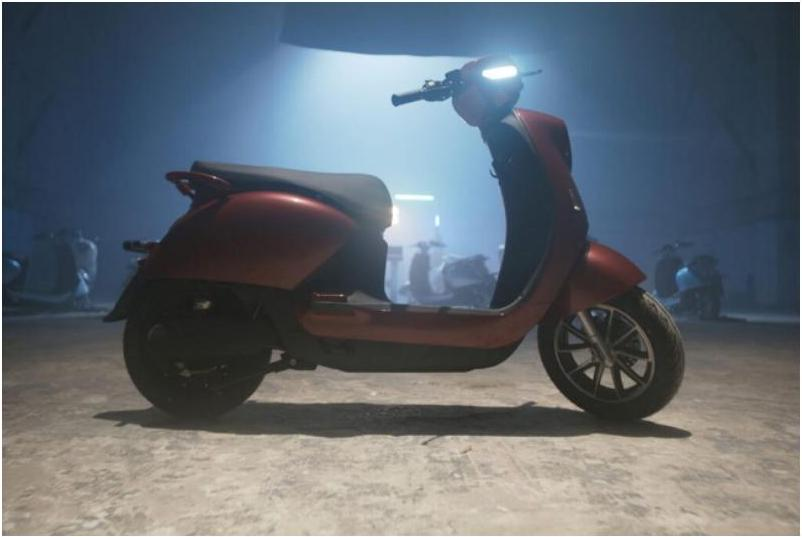
\includegraphics[alt={},max width=\textwidth]{5f5eb520-01ce-45b9-9641-42f0a6c20c83-01_537_802_1364_215}
\captionsetup{labelformat=empty}
\caption{Figure 1 - Le Liger $X$ à l'équilibre, sans béquille}
\end{center}
\end{figure}

\begin{figure}[h]
\begin{center}
  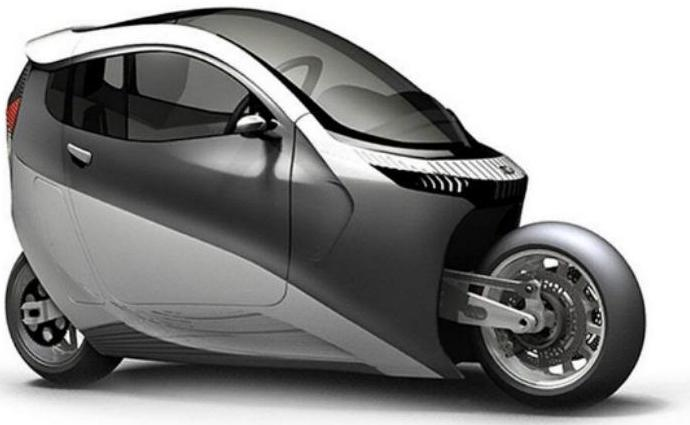
\includegraphics[alt={},max width=\textwidth]{5f5eb520-01ce-45b9-9641-42f0a6c20c83-01_425_690_1403_1142}
\captionsetup{labelformat=empty}
\caption{Figure 2 - Le Lit Motors AEV (véhicule électrique gyrostabilisé)}
\end{center}
\end{figure}

La vitesse de rotation d'une roue engendre un effet gyroscopique qui permet de la maintenir en équilibre, ce qui influe sur le pilotage du véhicule. En effet, au-dessus de $35 \mathrm{~km} \cdot \mathrm{~h}^{-1}$, un deux-roues est en équilibre grâce à l'effet gyroscopique de ses roues. Le contrôle de la trajectoire se fait alors en inclinant le deux-roues.

Lors d'une quantification des causes d'accidents de deux-roues motorisés faite en 2019, il a été démontré qu'un facteur aggravant est le défaut de maîtrise lors du freinage. En effet, les scooters de petite cylindrée utilisés majoritairement en milieu urbain ne sont que rarement équipés d'un système antiblocage des roues (ABS) et tout aussi rarement d'un système de couplage entre les actions des freins avant et arrière. C'est le mauvais dosage de ces actions qui conduit le plus souvent à la chute lors d'un évitement.

Dans ce contexte, il est nécessaire d'imaginer un système anti-chute pour éviter la perte d'équilibre. Le système, étudié ici, doit maintenir l'équilibre du scooter à basse vitesse en dépit des perturbations éventuelles et ne pas gêner la conduite quelle que soit la vitesse.

\footnotetext{\begin{enumerate}
  \item Rapport de situation sur la sécurité routière dans le monde, 2023, "Global status report on road safety 2023", OMS, \href{https://www.who.int/teams/social-determinants-of-health/safety-and-mobility/global-status-report-on-road-safety-2023}{https://www.who.int/teams/social-determinants-of-health/safety-and-mobility/global-status-report-on-road-safety-2023}
\end{enumerate}
}Stabiliser un véhicule à deux roues lors d'un trajet urbain, sans perturber la conduite sur route.

Afin de répondre à cet objectif, l'étude s'appuie sur le cahier des charges représenté par les contraintes exprimées au moyen du diagramme des exigences partiel de la figure 3.

\begin{figure}[h]
\begin{center}
  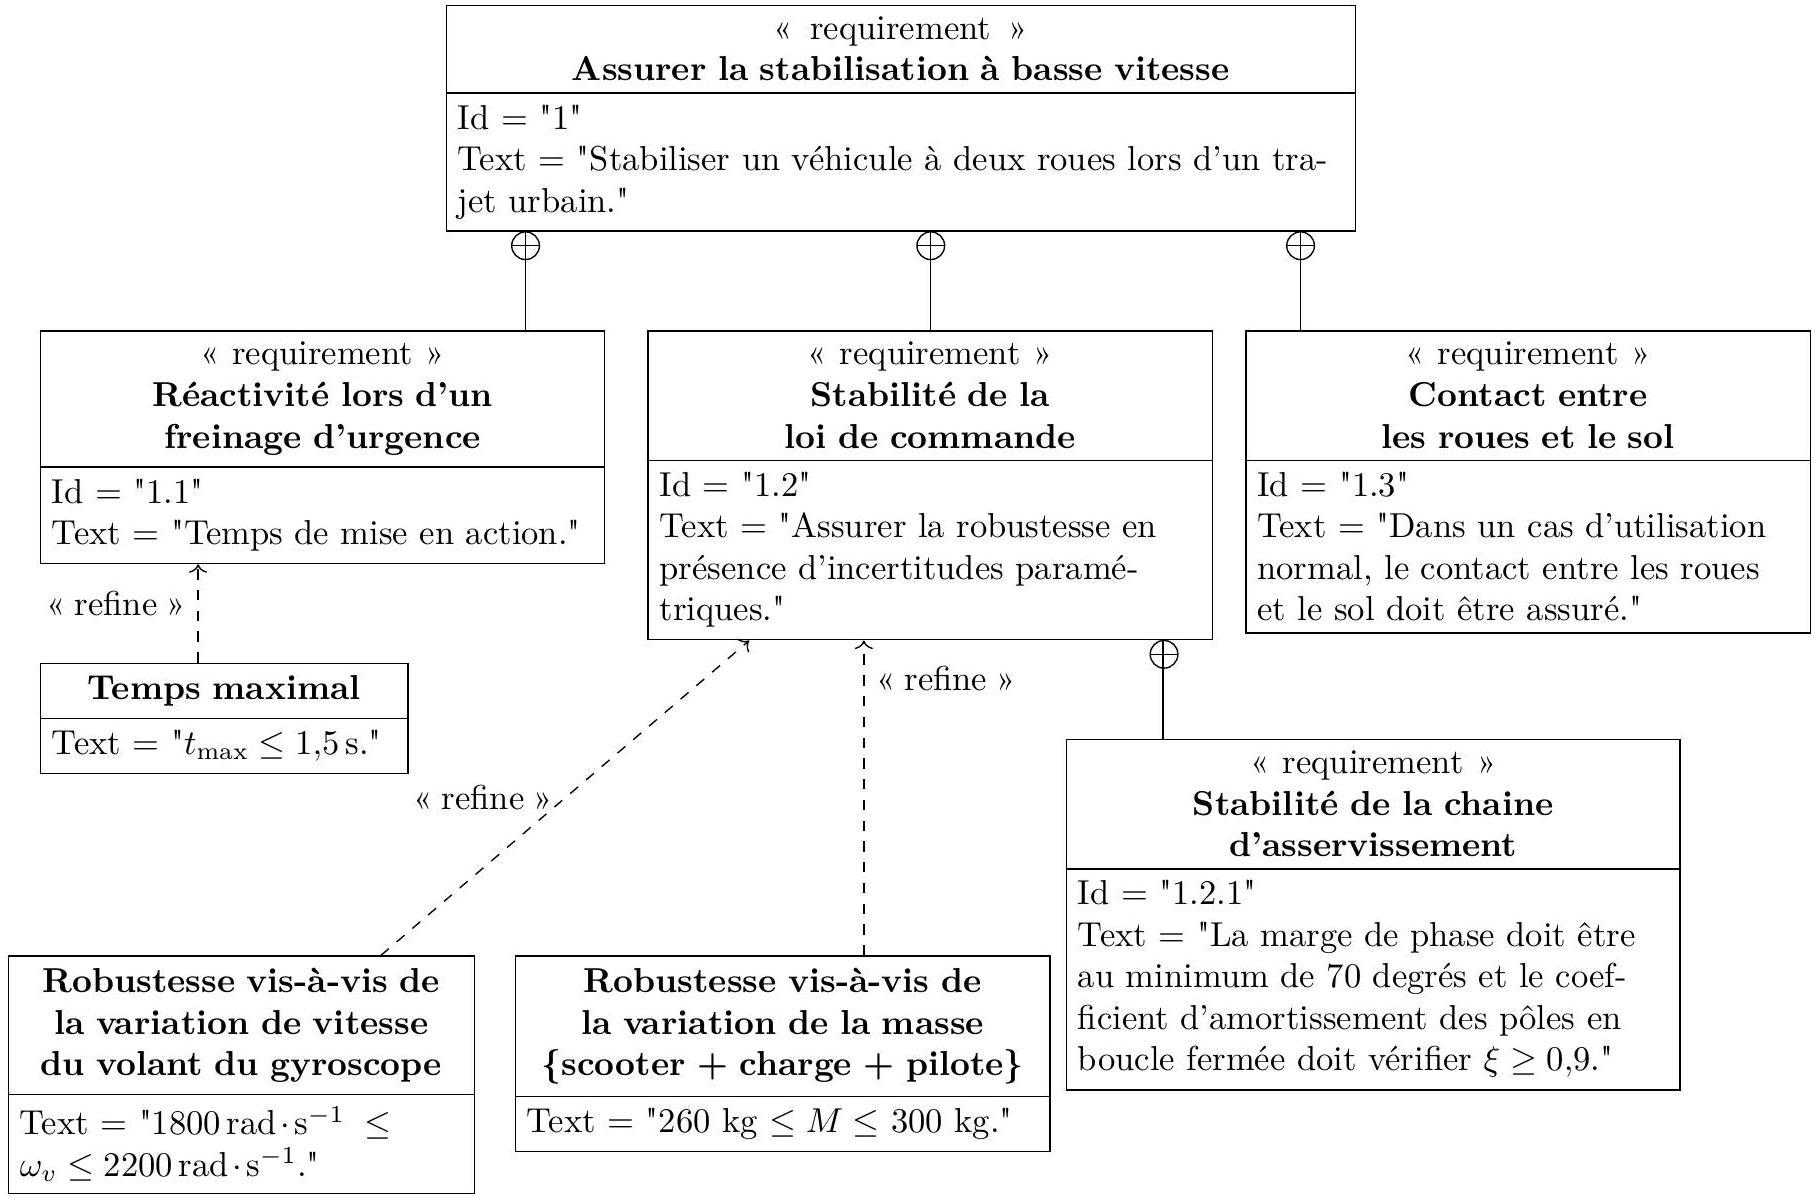
\includegraphics[alt={},max width=\textwidth]{5f5eb520-01ce-45b9-9641-42f0a6c20c83-02_1198_1816_457_140}
\captionsetup{labelformat=empty}
\caption{Figure 3 - Diagramme d'exigences partiel pour la stabilisation d'un deux-roues à basse vitesse}
\end{center}
\end{figure}

La solution retenue en vue de stabiliser le véhicule à deux roues fait appel à un actionneur gyroscopique piloté, fixé sur le cadre du véhicule. L'objectif de cette étude est alors d'imaginer une loi de commande stabilisante répondant aux contraintes exprimées par le diagramme des exigences partiel de la figure 3. En exploitant les mesures disponibles, cette loi de commande doit permettre de calculer le signal de pilotage de l'actionneur gyroscopique en vue de maintenir l'équilibre du véhicule.

La démarche de conception de la loi de commande nécessite de définir les modèles représentant le comportement du système, mais aussi de déterminer le temps de stabilisation maximal lors d'un freinage d'urgence en vue de vérifier la condition de réactivité pour cette phase de fonctionnement. Le calcul de ce temps maximal est une donnée importante car elle conditionne le temps de réponse à imposer aux chaînes d'asservissement de ce système.

\section{Partie A - Temps de stabilisation maximal pour la mise en action de l'assistance}
\begin{itemize}
  \item Objectif
\end{itemize}

Valider le temps disponible pour activer l'assistance lors d'un freinage de $50 \mathrm{~km} \cdot \mathrm{~h}^{-1}$ à $35 \mathrm{~km} \cdot \mathrm{~h}^{-1}$.

Le cahier des charges stipule que le système doit être suffisamment réactif lors d'un freinage d'urgence en milieu urbain. Afin de quantifier le temps maximal pour l'activation du système anti-chute, les hypothèses suivantes sont faites (en référence au paramétrage fourni en figure 4)

\begin{itemize}
  \item[-] la masse de l'ensemble $\Sigma=\{1+2+3+4\}$ est $M=280 \mathrm{~kg}$ avec comme poids de l'ensemble $P=M g$ ( $g=9,81 \mathrm{~m} \cdot \mathrm{~s}^{-2}$ l'accélération de la pesanteur);
  \item[-] le scooter et son pilote se déplacent en ligne droite à une vitesse initiale de $50 \mathrm{~km} \cdot \mathrm{~h}^{-1}$ (dans ce cas, la base $\mathcal{B}_{1}=\left(\vec{x}_{1}, \vec{y}_{1}, \vec{z}_{1}\right)$ est confondue avec la base $\left.\mathcal{B}_{0}=\left(\vec{x}_{0}, \vec{y}_{0}, \vec{z}_{0}\right)\right)$;
  \item[-] le risque de chute n'est possible qu'à une vitesse inférieure à $35 \mathrm{~km} \cdot \mathrm{~h}^{-1}$, vitesse à partir de laquelle l'effet gyroscopique des roues ne maintient plus naturellement l'ensemble à l'équilibre ;
  \item[-] le freinage n'est effectué que sur la roue avant (3), et le scooter est équipé de l'ABS assurant un roulement sans glissement (RSG) entre la roue avant et le sol;
  \item[-] le moteur ne fournit aucun couple sur la roue arrière ;
  \item[-] les contacts des roues avec le sol sont modélisés par des liaisons sphère-plan avec frottement (de normale $\vec{x}_{0}$ pour la roue arrière (4) et pour la roue avant (3)). Chaque roue roule sans glisser sur la route au niveau de son point de contact. Les actions mécaniques exercées par le sol sur les roues sont modélisées (en modélisation plane) par
$$
\mathscr{T}_{\mathrm{sol} \rightarrow 3}=\left\{N_{A} \vec{x}_{0}-T_{A} \vec{y}_{0}\right\}_{A} \quad \text { et } \quad \mathscr{T}_{\mathrm{sol} \rightarrow 4}=\left\{N_{B} \vec{x}_{0}-T_{B} \vec{y}_{0}\right\}_{B} ;
$$
  \item[-] l'ensemble (1) \{cadre du scooter + pilote (considéré comme infiniment rigide sur le scooter)\} est lié par le biais d'une liaison pivot d'axe $\left(O_{2}, \vec{x}_{2}\right)$ avec la fourche (2);
  \item[-] les deux roues du scooter (de centres $O_{3}$ et $O_{4}$ ) sont guidées en rotation par rapport à la fourche (2) à l'avant et à l'ensemble (1) à l'arrière du scooter;
  \item[-] le scooter se déplace en translation rectiligne à la vitesse $\vec{V}_{G \in 1 / 0}=v(t) \vec{y}_{0}$ et l'accélération $\gamma$ est telle que $\vec{\Gamma}_{G \in 1 / 0}=-\gamma \vec{y}_{0}$ (avec $G$ centre de gravité de l'ensemble $\Sigma$ );
  \item[-] le coefficient de frottement roue/sol est noté $f$ avec $f=0,6$ (cas défavorable d'une route dégradée) ;
  \item[-] pour cette étude, les masses et les inerties des roues sont négligées ;
  \item[-] le scooter étant en ligne droite, le paramétrage géométrique est le suivant
$$
\overrightarrow{O_{4} O_{3}}=L \vec{y}_{0} \quad \overrightarrow{A O_{3}}=\overrightarrow{B O_{4}}=R \vec{x}_{0} \quad \overrightarrow{O_{4} G}=h \vec{x}_{0}+a_{4} \vec{y}_{0} ;
$$
avec
$$
L=1350 \mathrm{~mm} \quad R=240 \mathrm{~mm} \quad h=570 \mathrm{~mm} \quad a_{4}=405 \mathrm{~mm} .
$$
\end{itemize}

Le paramétrage retenu pour l'étude du scooter et la modélisation à l'aide d'un graphe de liaisons sont fournis respectivement sur les figures 4 et 5 .

\begin{figure}[h]
\begin{center}
  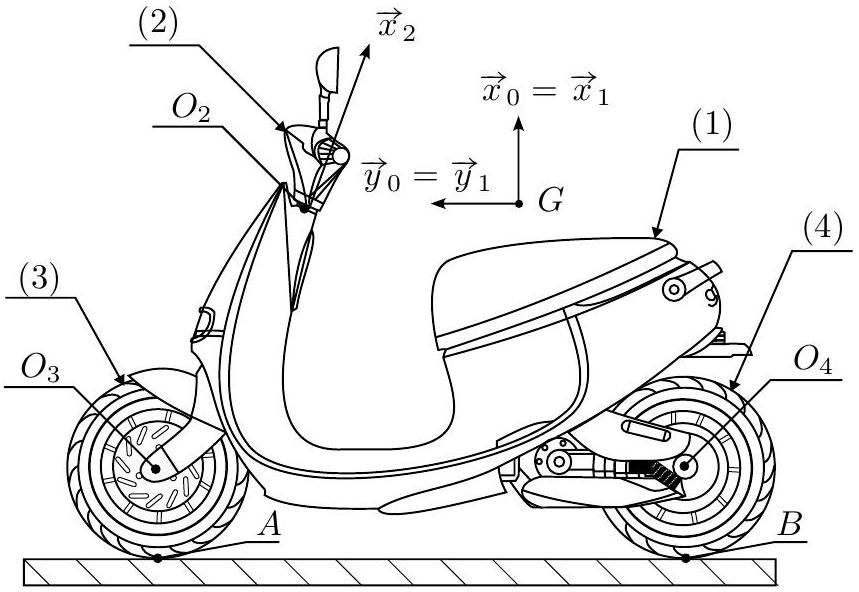
\includegraphics[alt={},max width=\textwidth]{5f5eb520-01ce-45b9-9641-42f0a6c20c83-03_592_859_1787_147}
\captionsetup{labelformat=empty}
\caption{Figure 4 - Paramétrage dimensionnel du scooter étudié en ligne droite}
\end{center}
\end{figure}

\begin{figure}[h]
\begin{center}
  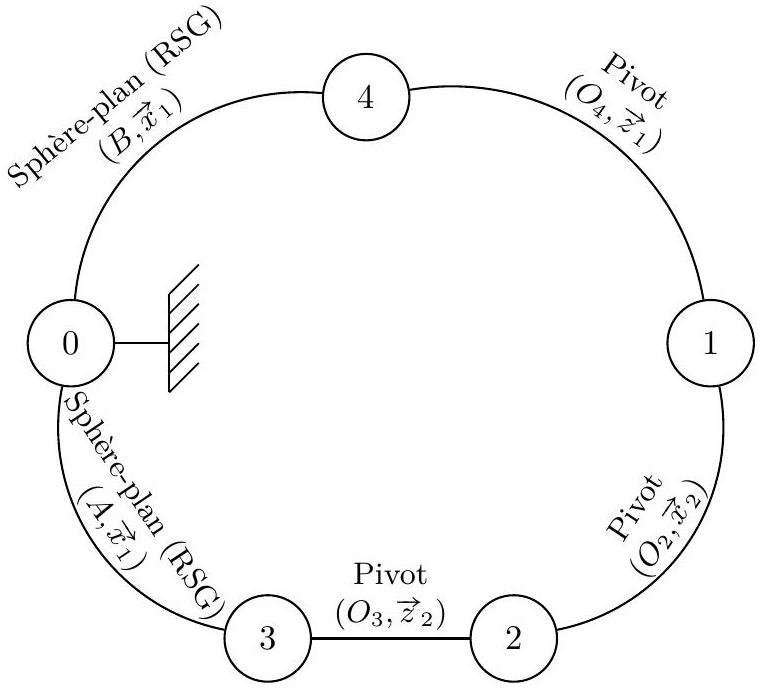
\includegraphics[alt={},max width=\textwidth]{5f5eb520-01ce-45b9-9641-42f0a6c20c83-03_688_763_1732_1131}
\captionsetup{labelformat=empty}
\caption{Figure 5 - Graphe de liaisons d'un scooter classique, sans dispositif de stabilisation}
\end{center}
\end{figure}

Q1. En isolant la roue arrière (4), démontrer que $T_{B}=0$.\\
Q2. En appliquant le principe fondamental de la dynamique à l'ensemble $\Sigma=\{1+2+3+4\}$, exprimer, sous forme littérale, $N_{A}, N_{B}$ et $T_{A}$ en fonction des accélérations $\gamma$ et $g$, de la masse $M$ et des données géométriques.

\begin{itemize}
  \item[Q3.] Vérifier si la roue arrière reste en contact du sol lors d'un tel freinage et conclure par rapport aux exigences du cahier des charges.
  \item[Q4.] Déterminer la valeur $\gamma_{\text {max }}$ de $\gamma$ permettant un freinage efficace, c'est-à-dire à la limite du glissement de la roue avant. Calculer alors le temps de freinage minimal, noté $t_{\text {fr }}$ permettant de réduire la vitesse de $50 \mathrm{~km} \cdot \mathrm{~h}^{-1}$ à $35 \mathrm{~km} \cdot \mathrm{~h}^{-1}$. Conclure par rapport aux exigences du cahier des charges.
\end{itemize}

Afin de faire face au risque de chute, une solution est d'implanter un système de gyrostabilisation se mettant en action dans le temps de freinage minimal obtenu précédemment. La conception et le réglage de ce système nécessitent, entre autres, de disposer d'un modèle de l'ensemble \{pilote + scooter\} valide à basse vitesse.

\section{Partie B - Modélisation comportementale à petite vitesse}
\begin{itemize}
  \item Objectif
\end{itemize}

Déterminer le modèle de comportement de l'ensemble \{pilote + scooter\} en milieu urbain et justifier l'utilité d'un système anti-chute par l'exploitation de ce modèle.

Le scooter suit initialement une trajectoire rectiligne et le paramétrage retenu est fourni figure 6.

\begin{figure}[h]
\begin{center}
  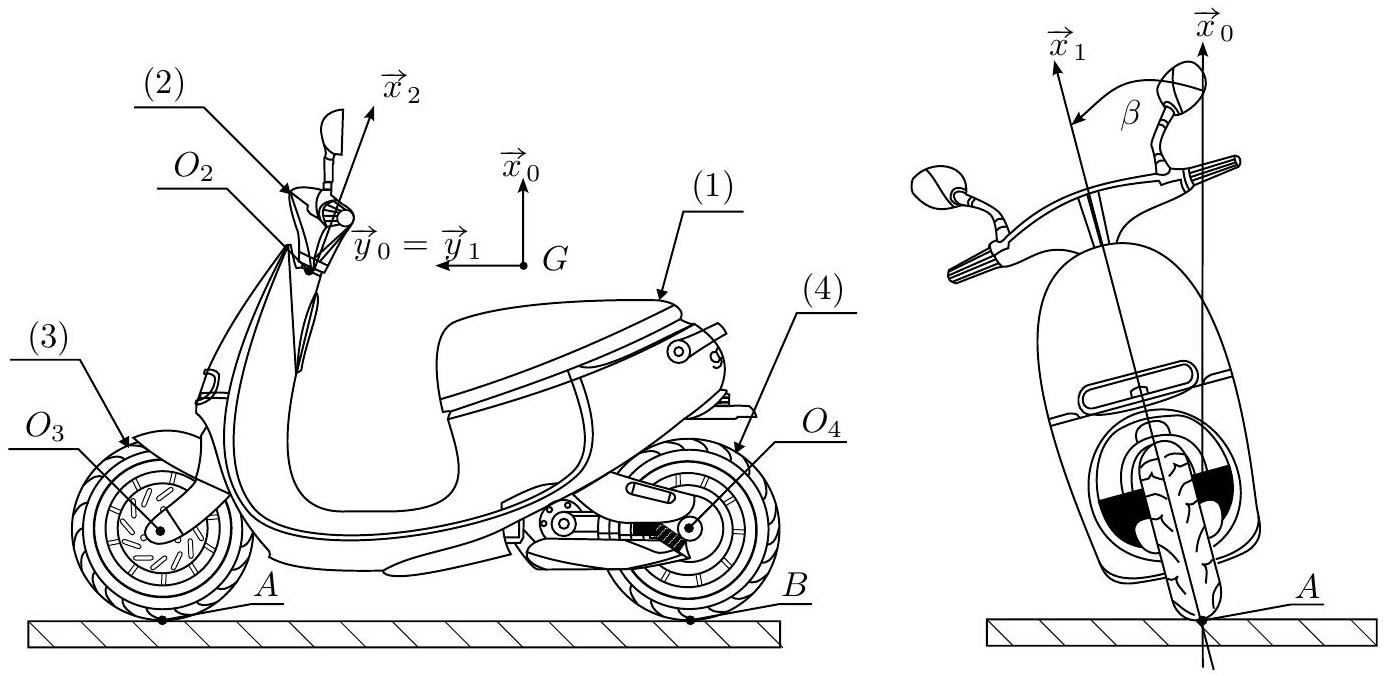
\includegraphics[alt={},max width=\textwidth]{5f5eb520-01ce-45b9-9641-42f0a6c20c83-04_676_1386_1003_342}
\captionsetup{labelformat=empty}
\caption{Figure 6 - Paramétrage du scooter}
\end{center}
\end{figure}

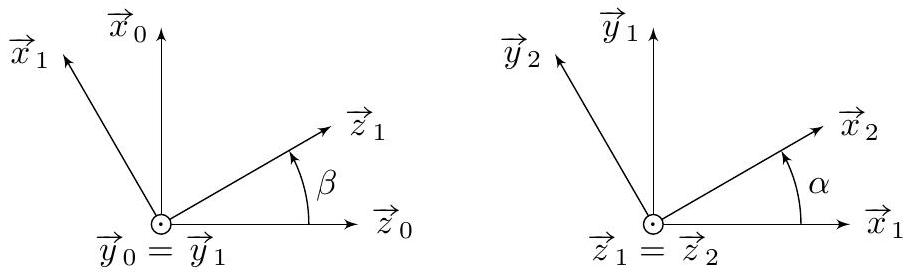
\includegraphics[max width=\textwidth, alt={}, center]{5f5eb520-01ce-45b9-9641-42f0a6c20c83-04_274_909_1783_577}\\
Avec

\begin{itemize}
  \item[]
  \begin{itemize}
    \item[-] le repère $\mathcal{R}_{0}$ lié au sol (0) $\left(O_{0}, \vec{x}_{0}, \vec{y}_{0}, \vec{z}_{0}\right)$ avec $\vec{x}_{0}$ vertical ascendant;
    \item[-] le repère $\mathcal{R}_{1}$ lié à l'ensemble \{cadre + pilote\} (1) $\left(G, \vec{x}_{1}, \vec{y}_{1}, \vec{z}_{1}\right)$ avec $\vec{y}_{1}=\vec{y}_{0}$. L'angle de roulis du cadre par rapport au sol (0) est noté $\beta=\left(\vec{x}_{0}, \vec{x}_{1}\right)$. La matrice d'inertie est notée
$$
I_{G, 1}=\left(\begin{array}{ccc}
A_{1} & -F_{1} & 0 \\
-F_{1} & B_{1} & 0 \\
0 & 0 & C_{1}
\end{array}\right)_{G, \mathcal{B}_{1}}
$$
avec $\mathcal{B}_{1}=\left(\vec{x}_{1}, \vec{y}_{1}, \vec{z}_{1}\right)$;
    \item[-] l'angle entre la fourche (2) de $\left(O_{2}, \vec{x}_{2}\right)$ par rapport au cadre (1) $\left(O_{2}, \vec{x}_{2}, \vec{y}_{2}, \vec{z}_{2}\right)$ est supposé nul au cours de cette partie de l'étude;
    \item[-] l'angle de chasse $\alpha=\left(\vec{x}_{1}, \vec{x}_{2}\right)$ avec $\alpha=-20^{\circ}$ représente l'angle entre l'axe de la colonne de direction et le vecteur $\vec{x}_{1}$. La masse de la fourche (2) est négligée;
  \end{itemize}
\end{itemize}

\begin{itemize}
  \item[-] le repère $\mathcal{R}_{3}$ lié à la roue avant (3) $\left(O_{3}, \vec{x}_{3}, \vec{y}_{3}, \vec{z}_{3}\right)$ avec $\vec{z}_{3}=\vec{z}_{2}$. L'angle de rotation $\theta_{3}$ de la roue avant (3) par rapport à la fourche (2) est paramétré tel que $\theta_{3}=\left(\vec{x}_{2}, \vec{x}_{3}\right)$. En considérant
  \begin{itemize}
    \item[-] $R$ le rayon de la roue;
    \item[-] $A$ le point de contact entre la roue et le sol. L'hypothèse de roulement sans glissement en $A$ est appliquée et $\overrightarrow{A O_{3}}=R \vec{x}_{1}$;
    \item[-] $d, h_{3}$ et $a_{3}$ tels que $\overrightarrow{O_{3} G}=-d \vec{y}_{2}+h_{3} \vec{x}_{1}-a_{3} \vec{y}_{1}$ ( $d$ est appelé le déport de la fourche);
    \item[-] la masse et l'inertie de la roue sont négligées.
  \end{itemize}
  \item[-] le repère $\mathcal{R}_{4}$ lié à la roue arrière (4) $\left(O_{4}, \vec{x}_{4}, \vec{y}_{4}, \vec{z}_{4}\right)$ avec $\vec{z}_{4}=\vec{z}_{1}$. L'angle de rotation $\theta_{4}$ de la roue arrière (4) par rapport au cadre (1) est paramétré tel que $\theta_{4}=\left(\vec{x}_{1}, \vec{x}_{4}\right)$. En considérant
  \begin{itemize}
    \item[-] $R$ le rayon de la roue;
    \item[-] $B$ le point de contact entre la roue et le sol. L'hypothèse de roulement sans glissement en $B$ est appliquée et $\overrightarrow{B O_{4}}=R \vec{x}_{1}$;
    \item[-] $h$ et $a_{4}$ tels que $\overrightarrow{O_{4} G}=h \vec{x}_{1}+a_{4} \vec{y}_{1}$;
    \item[-] la masse et l'inertie de la roue sont négligées.
  \end{itemize}
  \item[Q5.] Réaliser le bilan des actions mécaniques extérieures s'appliquant à l'ensemble $\Sigma=\{1+2+3+4\}$ et exprimer les torseurs des actions mécaniques correspondants.
  \item[Q6.] En appliquant les dérivations vectorielles nécessaires de $\overrightarrow{O_{0} G}$ par rapport à la base $\mathcal{B}_{0}$, calculer l'accélération au point $G$ de (1) par rapport à (0), notée $\vec{\Gamma}_{G, 1 / 0}$ et l'exprimer dans la base $\mathcal{B}_{1}$ en fonction de $\dot{\beta}, \ddot{\beta}, \dot{v}$ et des paramètres géométriques nécessaires.
  \item[Q7.] Après avoir calculé l'expression du moment dynamique en $G$ dans le mouvement de (1) par rapport à (0), déterminer l'expression du moment dynamique en $A$ suivant $\vec{y}_{1}$.
  \item[Q8.] Appliquer le théorème du moment dynamique en $A$ projeté sur le vecteur $\vec{y}_{1}$ et exprimer la relation de comportement dynamique du mouvement du scooter sous la forme $\ddot{\beta}=q(\beta)$ où $q(\beta)$ est une fonction dépendant de $\beta$ à préciser avec les différents paramètres existants.
\end{itemize}

Lors de l'étude du comportement du scooter suite à une légère modification de l'angle de roulis $\beta$, il est possible de paramétrer le système juste avant la prise en compte de cette perturbation en fonction des conditions initiales :

$$
\beta(0)=0 \quad \dot{\beta}(0)=\Omega_{0}
$$

En linéarisant la relation obtenue à la question Q8, l'équation différentielle peut alors être formulée comme suit :

$$
\ddot{\beta}(t)=K_{1} \beta(t)
$$

avec $K_{1}$ une constante positive.

\begin{itemize}
  \item[Q9.] En exploitant les propriétés de la transformation de Laplace, montrer que le comportement dynamique du scooter peut-être représenté sous la forme du schéma bloc de la figure 7 avec $c>0$ où $\beta(p)$ est la transformée de Laplace de $\beta(t)$ et $\Omega_{0}$ est assimilé à un signal externe. Préciser les expressions de $K$ et $c$.

\begin{figure}[h]
\begin{center}
      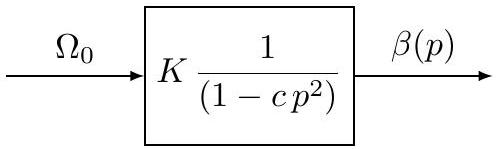
\includegraphics[alt={},max width=\textwidth]{5f5eb520-01ce-45b9-9641-42f0a6c20c83-05_149_496_2102_784}
\captionsetup{labelformat=empty}
\caption{Figure 7 - Modèle dynamique d'évolution de l'angle de roulis de l'ensemble \{pilote + scooter\}}
\end{center}
\end{figure}

  \item[Q10.] Conclure quant à la stabilité du scooter.
\end{itemize}

En exploitant le modèle de l'ensemble \{pilote + scooter\} établi précédemment, il est possible d'envisager la conception du système anti-chute actif fondé sur l'implantation d'un actionneur gyroscopique.

\section{Partie C - Modélisation de l'ensemble \{scooter+pilote+gyroscope\}}
\begin{itemize}
  \item Objectif
\end{itemize}

Établir un modèle de comportement dynamique du gyroscope implanté sur le scooter.

\section{I - Modélisation du gyroscope}
\begin{itemize}
  \item Objectif
\end{itemize}

Calculer le couple généré par le gyroscope piloté seul fixé sur le cadre.

Afin de stabiliser l'ensemble, un actionneur gyroscopique, comportant un volant d'inertie entraîné à vitesse de rotation constante $\omega_{v}$, est implanté sur le cadre du scooter. Le modèle retenu est présenté en figure 8. Une machine électrique permet de piloter l'angle $\psi$.

\begin{figure}[h]
\begin{center}
  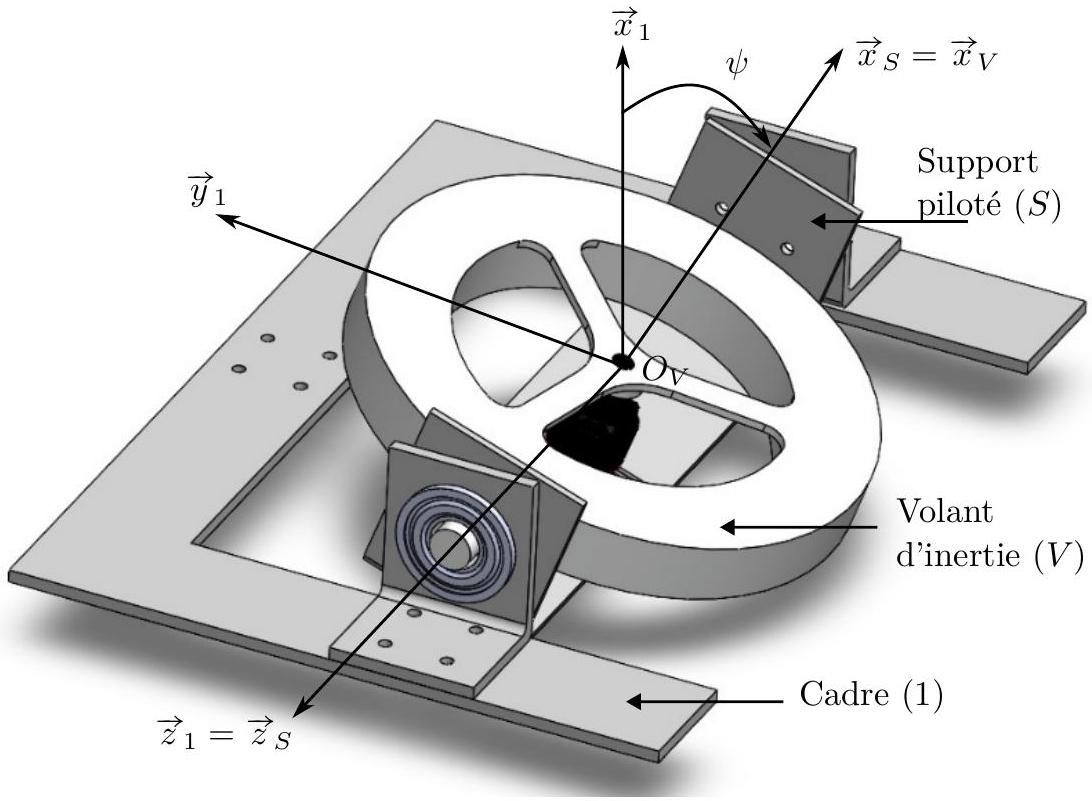
\includegraphics[alt={},max width=\textwidth]{5f5eb520-01ce-45b9-9641-42f0a6c20c83-06_801_1092_820_471}
\captionsetup{labelformat=empty}
\caption{Figure 8 - Modèle 3D du gyroscope}
\end{center}
\end{figure}

Le paramétrage suivant est retenu

\begin{itemize}
  \item[-] le repère $\mathcal{R}_{1}$, supposé galiléen, lié à l'ensemble \{cadre + pilote\} (1) en supposant la vitesse de l'ensemble constante et en ligne droite;
  \item[-] le repère $\mathcal{R}_{S}$ lié au support piloté $(S):\left(O_{V}, \vec{x}_{S}, \vec{y}_{S}, \vec{z}_{S}\right)$ avec $\vec{z}_{S}=\vec{z}_{1}$. L'angle de rotation du support piloté $(S)$ par rapport à l'ensemble \{cadre + pilote\} (1) est noté $\psi=\left(\vec{x}_{1}, \vec{x}_{S}\right)$. La masse de $(S)$ est négligée ;
  \item[-] le repère $\mathcal{R}_{V}$ lié au volant d'inertie $\left(O_{V}, \vec{x}_{V}, \vec{y}_{V}, \vec{z}_{V}\right)$ avec $\vec{x}_{V}=\vec{x}_{S}$. Avec
  \begin{itemize}
    \item[-] $\omega_{v}$ la vitesse de rotation du volant d'inertie $(V)$ par rapport au support piloté $(S)$ autour de $\left(O_{V}, \vec{x}_{S}\right)$, $\omega_{v}$ est supposée constante;
    \item[-] la matrice d'inertie du volant
$$
I_{O_{V}, V}=\left(\begin{array}{ccc}
A_{V} & 0 & 0 \\
0 & B_{V} & 0 \\
0 & 0 & B_{V}
\end{array}\right)_{O_{V}, \mathcal{B}_{S}}
$$
avec $\mathcal{B}_{S}=\left(\vec{x}_{S}, \vec{y}_{S}, \vec{z}_{S}\right)$;
    \item[-] le centre de gravité du volant $O_{V}$.
  \end{itemize}
\end{itemize}

Les actions mécaniques qui s'appliquent sur le gyroscope sont

\begin{itemize}
  \item[-] l'action de (1) sur (S) $\mathscr{T}_{1 \rightarrow S}=\left\{\begin{array}{c}\vec{F}_{1 S} \\ L_{1 S} \vec{x}_{S}+M_{1 S} \vec{y}_{S}\end{array}\right\}_{O_{V}}$;
  \item[-] l'action de la machine électrique sur $(S) \mathscr{T}_{\mathrm{m} \rightarrow S}=\left\{\begin{array}{c}\overrightarrow{0} \\ C_{m} \vec{z}_{S}\end{array}\right\}_{\forall P}$;
  \item[-] l'action de la pesanteur est négligée.
\end{itemize}

Pour la suite de l'étude, au regard des hypothèses mentionnées, le moment dynamique du support piloté est négligé par rapport à celui du volant d'inertie.

\begin{itemize}
  \item[Q11.] Réaliser le graphe de structure permettant de relier les solides (1), ( $S$ ) et $(V)$ en faisant intervenir l'ensemble des actions mécaniques agissant sur les solides $(S)$ et $(V)$.
  \item[Q12.] Proposer une démarche pour déterminer l'expression du couple $C_{m}$ sur le support piloté $(S)$ en fonction de l'accélération angulaire $\psi$.
  \item[Q13.] Calculer le moment cinétique de $(V)$ par rapport à l'ensemble (1) dans la base du repère $\mathcal{R}_{S}$ écrit au point $O_{V}$.
  \item[Q14.] En utilisant la démarche décrite question Q12, déterminer l'expression du couple $C_{m}$ sur le support piloté $(S)$ en fonction de l'accélération angulaire $\ddot{\psi}$.
\end{itemize}

En complément de cette partie, une application du théorème du moment dynamique sur le scooter complet permet d'aboutir à un modèle dynamique de l'ensemble \{pilote + scooter + gyroscope\} dont la grandeur de commande est le couple de la machine électrique $C_{m}$. Ce modèle est exploité dans la suite pour étudier une loi de commande stabilisante du système.

\section{II - Étude d'une loi de commande avec un retour sur l'angle de roulis}
\begin{itemize}
  \item Objectif
\end{itemize}

Étudier la stabilité de l'ensemble en exploitant un retour d'information sur l'angle de roulis du scooter.

En faisant l'hypothèse que l'ensemble \{pilote + scooter + gyroscope\} se déplace à basse vitesse et en ligne droite ( $\beta \approx 0$ et $\psi \approx 0$ ), l'équation comportementale utilisée est :


\begin{equation*}
\left(I_{1 y}+B_{V}\right) \ddot{\beta}(t)=-A_{V} \omega_{v} \dot{\psi}(t)+M g h_{2} \beta(t) \tag{1}
\end{equation*}


avec $I_{1 y}$ le moment d'inertie de l'ensemble (1) autour de $\vec{y}_{1}$.

L'étude du gyroscope conduit à l'équation (2) reliant le couple $C_{m}$ à l'angle $\beta$ :


\begin{equation*}
C_{m}(t)+A_{V} \omega_{v} \dot{\beta}(t)=B_{V} \ddot{\psi}(t) \tag{2}
\end{equation*}


L'ensemble des équations et l'utilisation d'un correcteur proportionnel noté $K_{\text {cor }}$ conduisent au schéma bloc de la structure asservie représentée figure 9.

\begin{figure}[h]
\begin{center}
  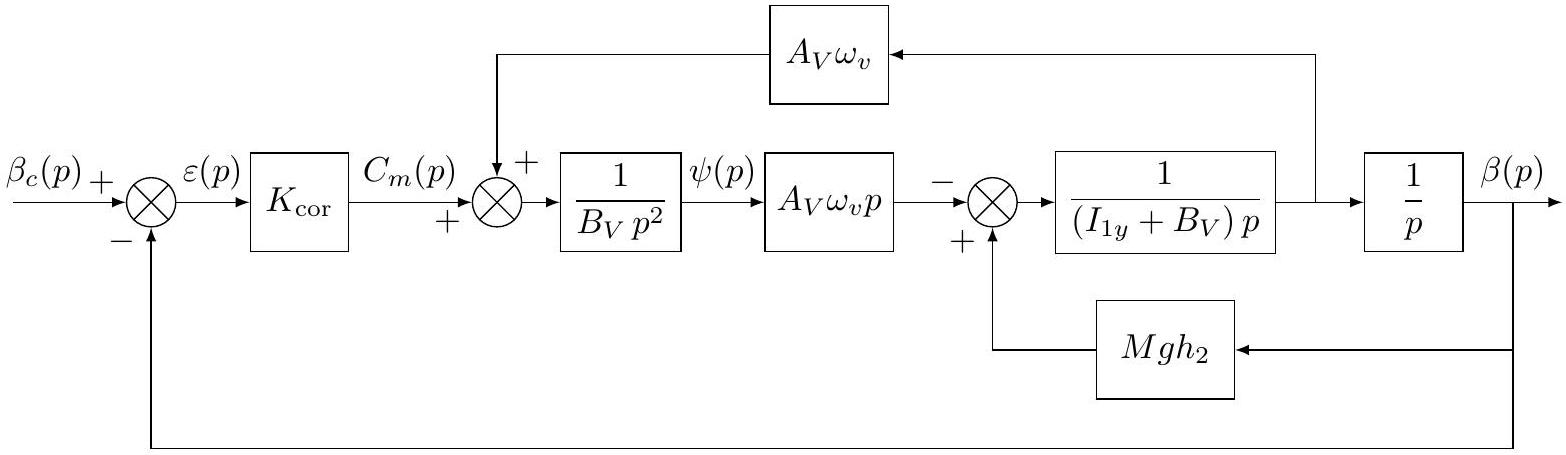
\includegraphics[alt={},max width=\textwidth]{5f5eb520-01ce-45b9-9641-42f0a6c20c83-07_455_1566_1771_255}
\captionsetup{labelformat=empty}
\caption{Figure 9 - Schéma bloc de l'asservissement de l'angle de roulis $\beta$ avec un correcteur proportionnel}
\end{center}
\end{figure}

\begin{itemize}
  \item[Q15.] Exprimer sous forme canonique la fonction de transfert en boucle fermée $\frac{\beta(p)}{\beta_{c}(p)}$.
  \item[Q16.] Conclure sur le comportement du scooter gyrostabilisé avec une correction proportionnelle seule et sur la capacité de ce système à répondre au cahier des charges fourni dans le diagramme des exigences.
\end{itemize}

Par la suite, afin de répondre à l'ensemble des exigences du cahier des charges, une nouvelle loi de commande est envisagée en supposant que des mesures complémentaires sont disponibles.

\section{Partie D - Étude de la loi de commande}
\begin{itemize}
  \item Objectif
\end{itemize}

Régler les paramètres d'une loi de commande permettant de stabiliser le comportement du scooter.

\section{I - Mise en place d'une loi de commande stabilisante}
\begin{itemize}
  \item Objectif
\end{itemize}

Calculer les paramètres d'une loi de commande en exploitant les mesures de l'angle de roulis $\beta$, de la dérivée de l'angle de roulis $\dot{\beta}$ et de l'angle $\psi$ du volant.

Afin d'assurer la stabilisation et les performances définies par le diagramme des exigences, la structure proposée en figure 10 est utilisée où $k_{1}, k_{2}$ et $k_{3}$ sont trois gains à déterminer.

\begin{figure}[h]
\begin{center}
  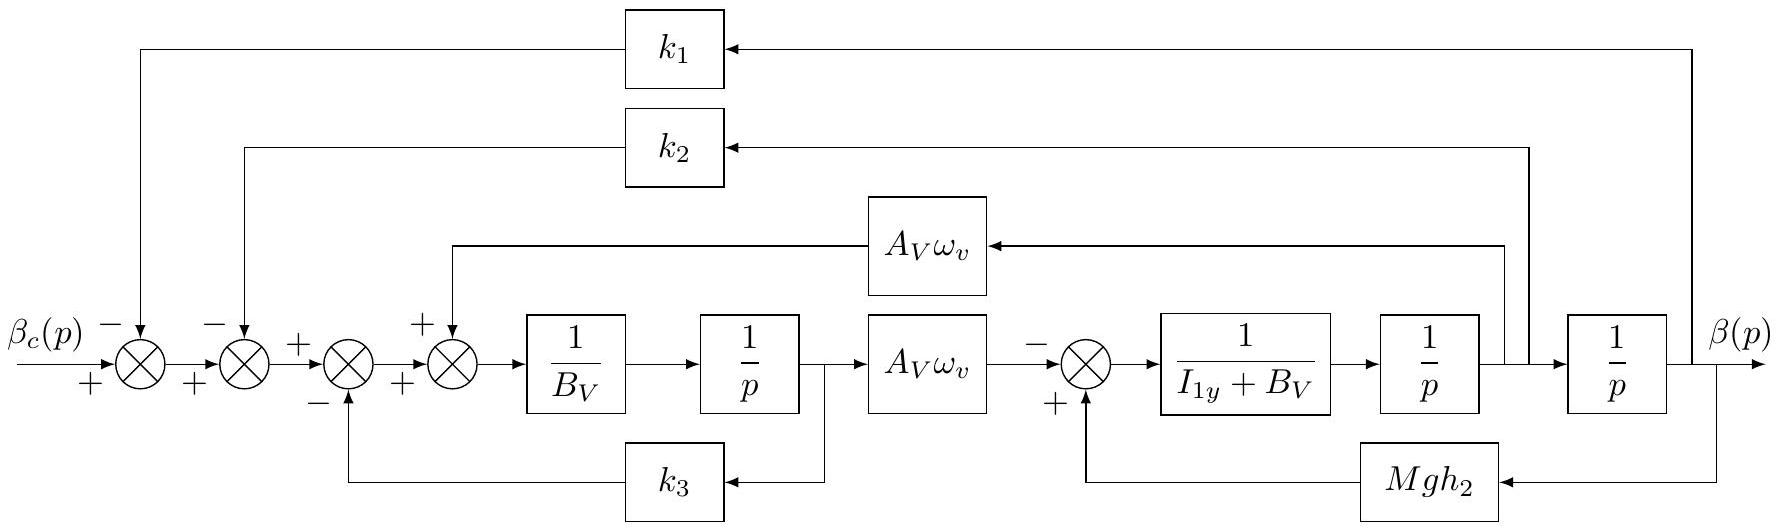
\includegraphics[alt={},max width=\textwidth]{5f5eb520-01ce-45b9-9641-42f0a6c20c83-08_529_1778_825_152}
\captionsetup{labelformat=empty}
\caption{Figure 10 - Schéma bloc de l'asservissement de l'angle de roulis $\beta$ avec exploitation de trois mesures}
\end{center}
\end{figure}

Au regard des exigences attendues, il est souhaitable que la chaîne de stabilisation du scooter ait un temps de réponse inférieur au temps de mise en action. Pour un temps d'établissement $t_{e}=0,5 \mathrm{~s}$, en exploitant la relation approchée $\omega_{0} t_{e} \approx 3$, il est décidé de placer les pôles $p_{1}, p_{2}$ et $p_{3}$ du système asservi en angle de roulis $\beta$ aux emplacements $p_{1,2}=-\omega_{0}\left(\xi \pm i \sqrt{1-\xi^{2}}\right)$ et $p_{3}=-60 \mathrm{~s}^{-1}$ avec $\omega_{0}=6 \mathrm{rad} \cdot \mathrm{s}^{-1}$ et $\xi=0,9$.\\
Il est donc nécessaire de déterminer les valeurs de $k_{1}, k_{2}$ et $k_{3}$ de façon à vérifier que les valeurs des emplacements polaires en boucle fermée correspondent aux valeurs retenues précédemment.

Q17. Établir l'expression de la fonction de transfert en boucle fermée $H(p)$ et la mettre sous la forme :

$$
H(p)=\frac{\beta(p)}{\beta_{c}(p)}=\frac{A_{V} \omega_{v}}{A\left(k_{1}, k_{3}\right)+B\left(k_{2}\right) p-C\left(k_{3}\right) p^{2}-D p^{3}}
$$

Préciser les termes $A, B, C$ et $D$ en fonction de $k_{1}, k_{2}, k_{3}$ et des paramètres du système.\\
Afin que les pôles $p_{i}$ souhaités précédemment soient obtenus, l'équation (3) doit être vérifiée :


\begin{equation*}
A\left(k_{1}, k_{3}\right)+B\left(k_{2}\right) p_{i}-C\left(k_{3}\right) p_{i}^{2}-D p_{i}^{3}=0 \quad \forall p_{i} \tag{3}
\end{equation*}


Q18. Reformuler l'équation (3) sous la forme :


\begin{equation*}
E_{0}\left(p_{i}\right)+E_{1}\left(p_{i}\right) k_{1}+E_{2}\left(p_{i}\right) k_{2}+E_{3}\left(p_{i}\right) k_{3}=0 \tag{4}
\end{equation*}


Préciser les expressions des fonctions $E_{0}, E_{1}, E_{2}$ et $E_{3}$.\\
Pour la suite, $E_{0}, E_{1}, E_{2}$ et $E_{3}$ s'écrivent sous la forme :

$$
\left\{\begin{array}{l}
E_{0}\left(p_{i}\right)=e_{01} p_{i}-e_{03} p_{i}^{3} \\
E_{1}\left(p_{i}\right)=e_{10} \\
E_{2}\left(p_{i}\right)=e_{21} p_{i} \\
E_{3}\left(p_{i}\right)=e_{30}-e_{32} p_{i}^{2}
\end{array}\right.
$$

L'équation (4) appliquée à chacun des pôles permet de poser le système suivant :

$$
\left\{\begin{array}{l}
E_{1}\left(p_{1}\right) k_{1}+E_{2}\left(p_{1}\right) k_{2}+E_{3}\left(p_{1}\right) k_{3}=-E_{0}\left(p_{1}\right) \\
E_{1}\left(p_{2}\right) k_{1}+E_{2}\left(p_{2}\right) k_{2}+E_{3}\left(p_{2}\right) k_{3}=-E_{0}\left(p_{2}\right) \\
E_{1}\left(p_{3}\right) k_{1}+E_{2}\left(p_{3}\right) k_{2}+E_{3}\left(p_{3}\right) k_{3}=-E_{0}\left(p_{3}\right)
\end{array}\right.
$$

Ce système est un système linéaire à coefficients complexes en fonction de $k_{1}, k_{2}$ et $k_{3}$. Il peut donc se mettre sous la forme matricielle $A L=B$ avec :

$$
A=\left(\begin{array}{lll}
E_{1}\left(p_{1}\right) & E_{2}\left(p_{1}\right) & E_{3}\left(p_{1}\right) \\
E_{1}\left(p_{2}\right) & E_{2}\left(p_{2}\right) & E_{3}\left(p_{2}\right) \\
E_{1}\left(p_{3}\right) & E_{2}\left(p_{3}\right) & E_{3}\left(p_{3}\right)
\end{array}\right) \quad ; \quad L=\left(\begin{array}{c}
k_{1} \\
k_{2} \\
k_{3}
\end{array}\right) \quad \text { et } \quad B=\left(\begin{array}{c}
-E_{0}\left(p_{1}\right) \\
-E_{0}\left(p_{2}\right) \\
-E_{0}\left(p_{3}\right)
\end{array}\right)
$$

Q19. À l'aide de la liste (non exhaustive) de fonctions et d'opérations du langage Python de l'annexe 1, compléter le code ci-dessous en vue

\begin{itemize}
  \item[-] de créer les matrices $A$ et $B$ définies précédemment;
  \item[-] de réaliser la résolution de ce système linéaire dont la solution est notée $L$.
  \item[1] import numpy as np
  \item[2] P=[p1,p2,p3]
  \item[] $3 \mathrm{E}=[\mathrm{e} 01, \mathrm{e} 03, \mathrm{e} 10, \mathrm{e} 21, \mathrm{e} 30, \mathrm{e} 32]$
\end{itemize}

Les valeurs $p 1, p 2, p 3, e 01, e 03, e 10, e 21$, e30 et e32 sont déjà affectées en mémoire.

La résolution renvoie la valeur de $L$ suivante :

$$
\begin{aligned}
& {[[-1.28887686 \mathrm{e}+02-4.09276709 \mathrm{e}-14 \mathrm{j}]} \\
& {[-1.56241539 \mathrm{e}+01-1.11022302 \mathrm{e}-16 \mathrm{j}]} \\
& [3.18600000 \mathrm{e}-02-2.16840434 \mathrm{e}-19 \mathrm{j}]]
\end{aligned}
$$

Q20. Donner les valeurs de $k_{1}, k_{2}$ et $k_{3}$ à retenir.

La réponse temporelle à un échelon de consigne d'amplitude 0,01 rad est donnée figure 11 (la figure de droite est un zoom de la figure de gauche).

\begin{figure}[h]
\begin{center}
  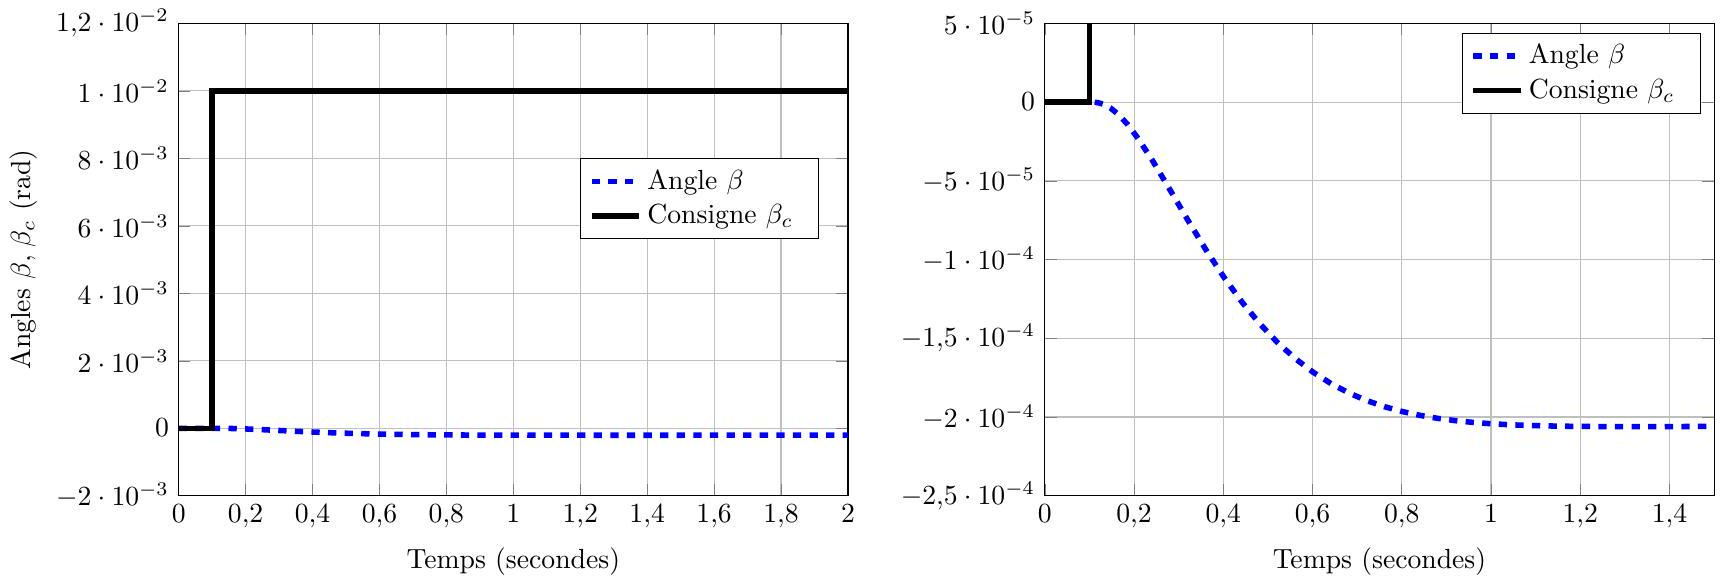
\includegraphics[alt={},max width=\textwidth]{5f5eb520-01ce-45b9-9641-42f0a6c20c83-09_585_1725_1704_176}
\captionsetup{labelformat=empty}
\caption{Figure 11 - Réponse temporelle du système bouclé pour un échelon de consigne d'amplitude 0,01 rad}
\end{center}
\end{figure}

Q21. Analyser et commenter les propriétés de la réponse obtenue.

Afin d'améliorer l'équilibre du scooter, le cahier des charges fourni en figure 3 est complété par une exigence de précision : l'écart en régime permanent doit être nul vis-à-vis de consignes en échelon.

Q22. Un gain proportionnel de pré-compensation est alors ajouté selon le schéma bloc de la figure 12. Proposer la valeur numérique de $K_{g}$ permettant d'assurer l'exigence de précision.

\begin{figure}[h]
\begin{center}
  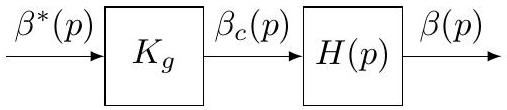
\includegraphics[alt={},max width=\textwidth]{5f5eb520-01ce-45b9-9641-42f0a6c20c83-10_110_507_130_781}
\captionsetup{labelformat=empty}
\caption{Figure 12 - Schéma bloc du système stabilisé en roulis $\beta$ avec pré-compensateur}
\end{center}
\end{figure}

Avec ce gain, la réponse temporelle du système en boucle fermée à un échelon de consigne $\beta^{*}(t)$ d'amplitude 0,01 rad est donnée sur la figure 13.

\begin{figure}[h]
\begin{center}
  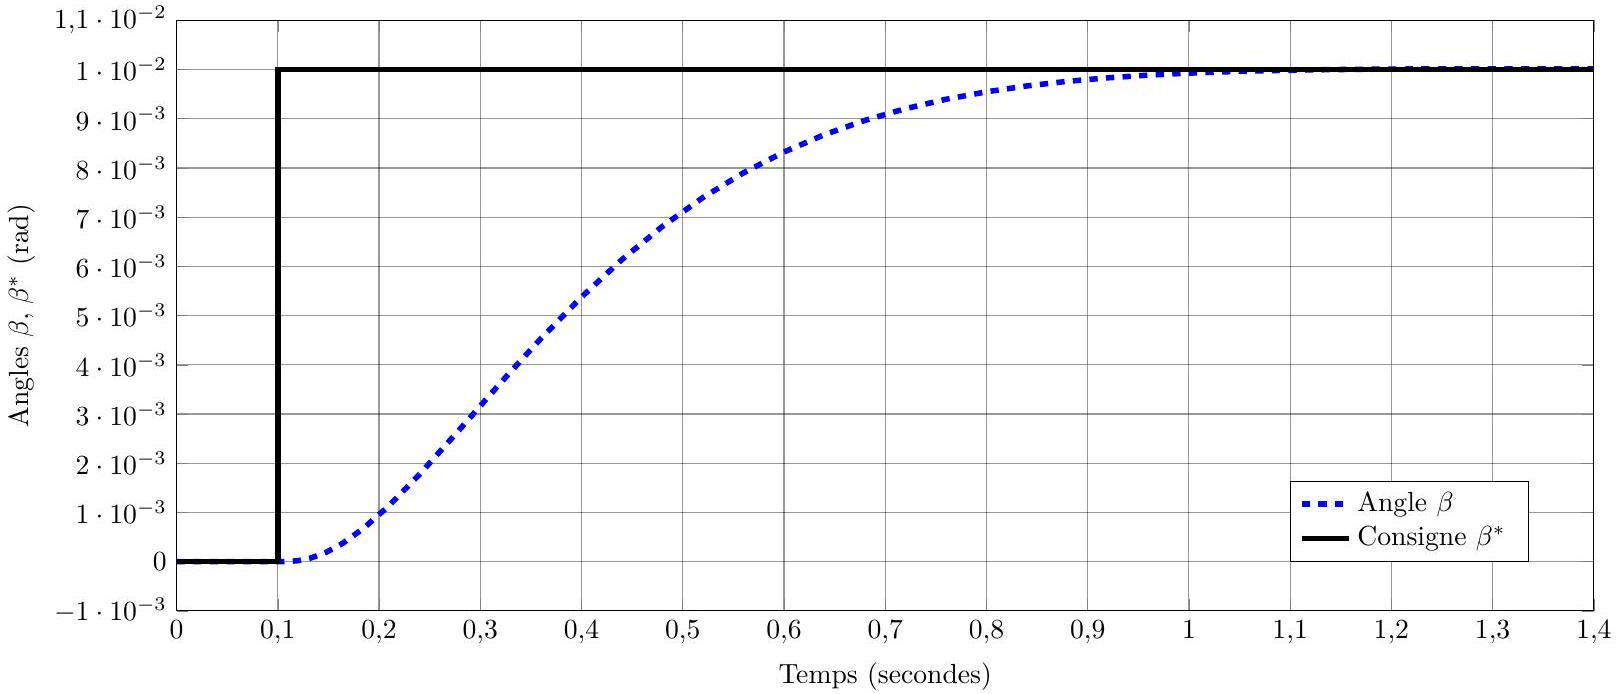
\includegraphics[alt={},max width=\textwidth]{5f5eb520-01ce-45b9-9641-42f0a6c20c83-10_694_1617_484_224}
\captionsetup{labelformat=empty}
\caption{Figure 13 - Réponse temporelle du système bouclé pour un échelon de consigne d'amplitude 0,01 rad avec le gain de pré-compensation $K_{g}$ adapté}
\end{center}
\end{figure}

\section{II - Analyse de la robustesse paramétrique}
\begin{itemize}
  \item Objectif
\end{itemize}

Analyser le comportement du scooter gyrostabilisé vis-à-vis des incertitudes paramétriques des modèles et relatives aux variations de la vitesse du volant du gyroscope et de la masse de l'ensemble.

Les paramètres de la loi de commande ont été déterminés pour une vitesse du volant de $2000 \mathrm{rad} \cdot \mathrm{s}^{-1}$ et une masse de l'ensemble \{scooter + pilote + gyroscope\} de 280 kg. En pratique, les valeurs de ces paramètres sont incertaines. Aussi, une étude en simulation est réalisée pour analyser l'effet de la variation des valeurs de ces paramètres au voisinage de leurs valeurs nominales. Les figures 14 et 15 montrent les résultats obtenus en réponse à un échelon de consigne d'amplitude 0,01 rad

\begin{itemize}
  \item[-] la figure 14 montre les résultats obtenus pour deux valeurs différentes de la vitesse du volant $\omega_{v} \in\{1800 ; 2200\} \mathrm{rad} \cdot \mathrm{s}^{-1}$;
  \item[-] la figure 15 montre les résultats obtenus pour deux valeurs différentes de la masse de l'ensemble $M \in\{260 ; 300\} \mathrm{kg}$.
\end{itemize}

\begin{figure}[h]
\begin{center}
  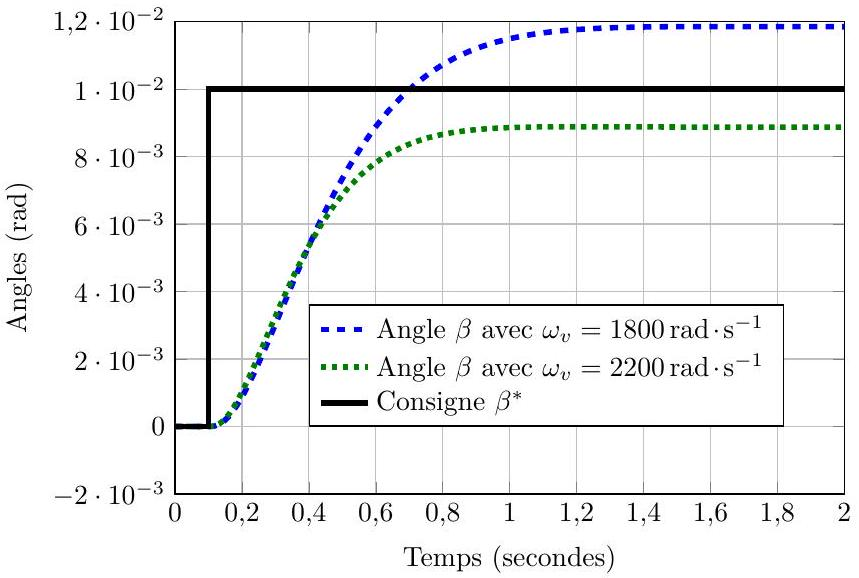
\includegraphics[alt={},max width=\textwidth]{5f5eb520-01ce-45b9-9641-42f0a6c20c83-10_578_859_2092_151}
\captionsetup{labelformat=empty}
\caption{Figure 14 - Effet de la variation de la vitesse du volant}
\end{center}
\end{figure}

\begin{figure}[h]
\begin{center}
  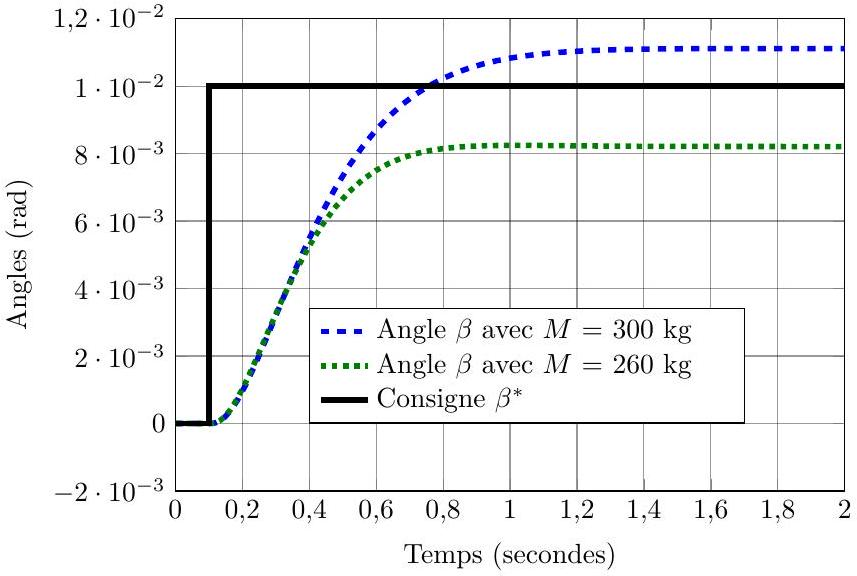
\includegraphics[alt={},max width=\textwidth]{5f5eb520-01ce-45b9-9641-42f0a6c20c83-10_576_857_2095_1039}
\captionsetup{labelformat=empty}
\caption{Figure 15 - Effet de la variation de la masse}
\end{center}
\end{figure}

Afin de pallier cette sensibilité paramétrique, la structure précédente est complétée avec un correcteur intégralproportionnel (IP) selon le schéma bloc de la figure 16 où $\beta_{\text {ref }}$ est la nouvelle consigne de référence. Il est rappelé que les pôles de $H(p)$ sont :

$$
p_{1}=-\omega_{0}\left(\xi+i \sqrt{1-\xi^{2}}\right) \quad p_{2}=-\omega_{0}\left(\xi-i \sqrt{1-\xi^{2}}\right) \quad p_{3}=-60 \mathrm{~s}^{-1}
$$

avec $\omega_{0}=6 \mathrm{rad} \cdot \mathrm{s}^{-1}$ et $\xi=0,9$.

\begin{figure}[h]
\begin{center}
  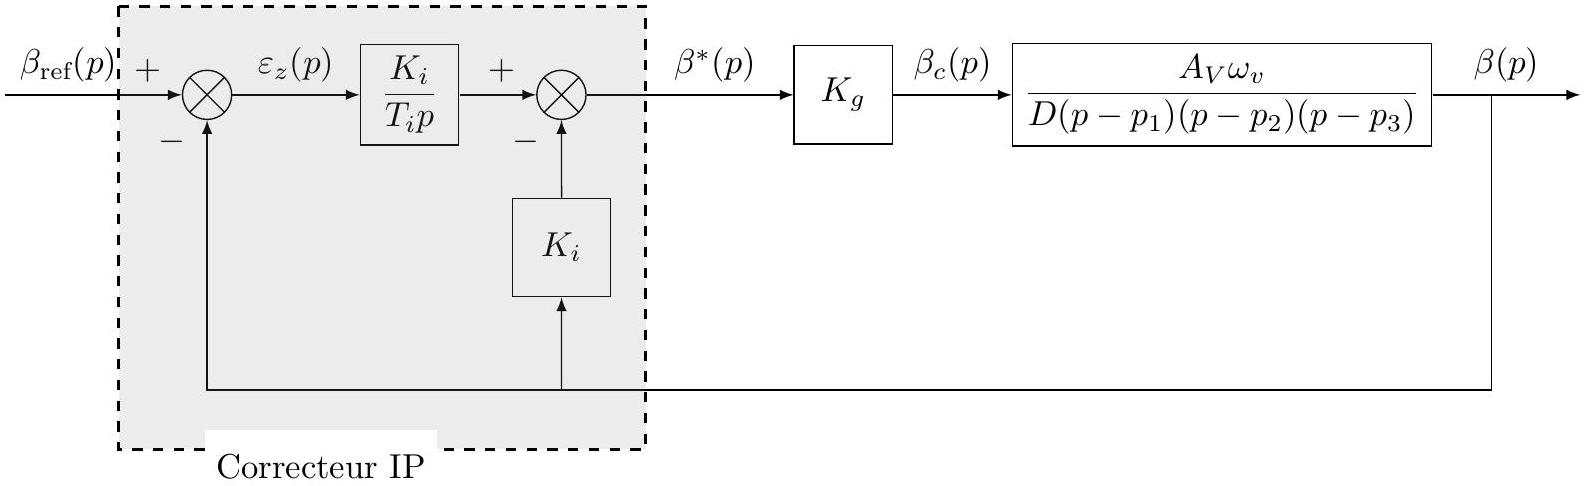
\includegraphics[alt={},max width=\textwidth]{5f5eb520-01ce-45b9-9641-42f0a6c20c83-11_486_1585_450_241}
\captionsetup{labelformat=empty}
\caption{Figure 16 - Schéma bloc de l'asservissement complet}
\end{center}
\end{figure}

Le choix des valeurs des paramètres $K_{i}$ et $T_{i}$ doit permettre d'assurer les exigences suivantes

\begin{itemize}
  \item[-] pulsation de coupure à 0 dB en boucle ouverte $\omega_{c_{\text {ext }}}=4 \mathrm{rad} \cdot \mathrm{s}^{-1}$;
  \item[-] marge de phase $\Delta \Phi \geq 70^{\circ}$.
\end{itemize}

Pour une telle structure de commande, la fonction de transfert en boucle ouverte est définie à partir du schéma bloc de la figure 17 par la relation $H_{b o}(p)=-\frac{S(p)}{\beta^{*}(p)}$.

\begin{figure}[h]
\begin{center}
  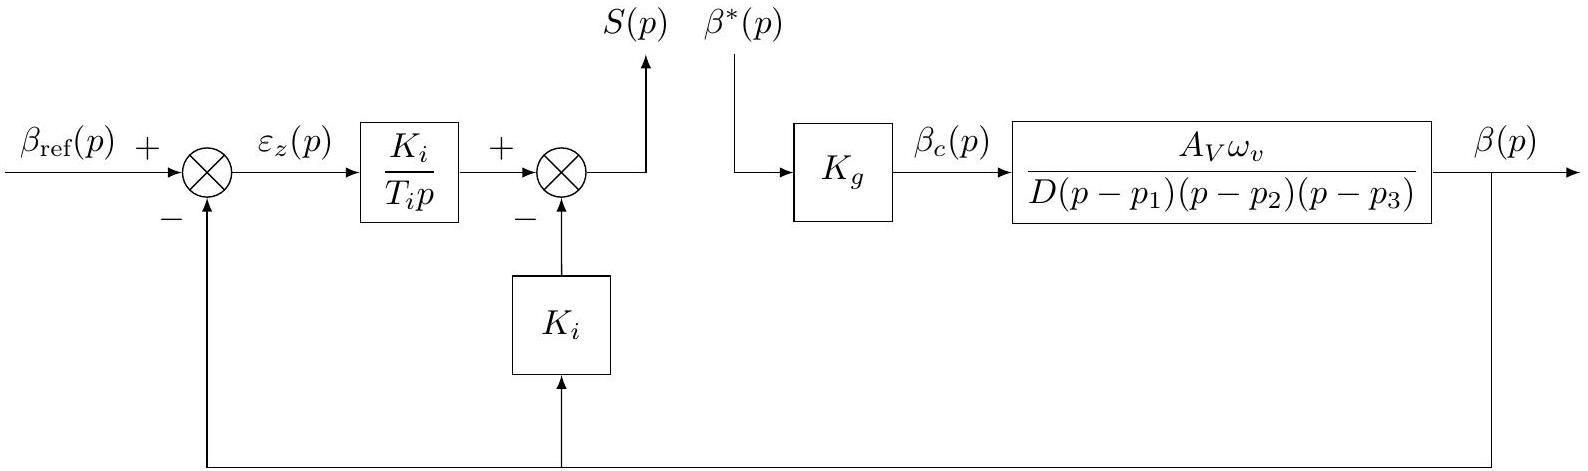
\includegraphics[alt={},max width=\textwidth]{5f5eb520-01ce-45b9-9641-42f0a6c20c83-11_471_1588_1419_241}
\captionsetup{labelformat=empty}
\caption{Figure 17 - Schéma bloc pour le calcul de la fonction de transfert en boucle ouverte}
\end{center}
\end{figure}

\begin{itemize}
  \item[Q23.] Déterminer la fonction de transfert en boucle ouverte $H_{b o}$ en fonction de $K_{i}, T_{i}, K_{g}$ et $H(p)=\frac{\beta(p)}{\beta_{c}(p)}$.
  \item[Q24.] En exploitant le diagramme de Bode de la fonction de transfert $\frac{\beta(p)}{\beta^{*}(p)}=K_{g} H(p)$ donné sur la figure 18, montrer que pour atteindre la marge de phase souhaitée le temps d'action intégrale $T_{i}$ doit vérifier $T_{i} \geq 0,3 \mathrm{~s}$.
  \item[Q25.] Pour la valeur minimale du temps d'action intégrale $T_{i}=0,3 \mathrm{~s}$, déterminer la valeur du gain $K_{i}$ permettant de vérifier les deux exigences.
\end{itemize}

Avec les valeurs des paramètres du correcteur $K_{i}$ et $T_{i}$ déterminées, le diagramme de Bode en boucle ouverte corrigée est donné sur le tracé de la figure 18.

\begin{itemize}
  \item[Q26.] En exploitant ce tracé, vérifier si les exigences imposées sont assurées et conclure sur la stabilité du système ainsi bouclé.
\end{itemize}

\begin{figure}[h]
\begin{center}
  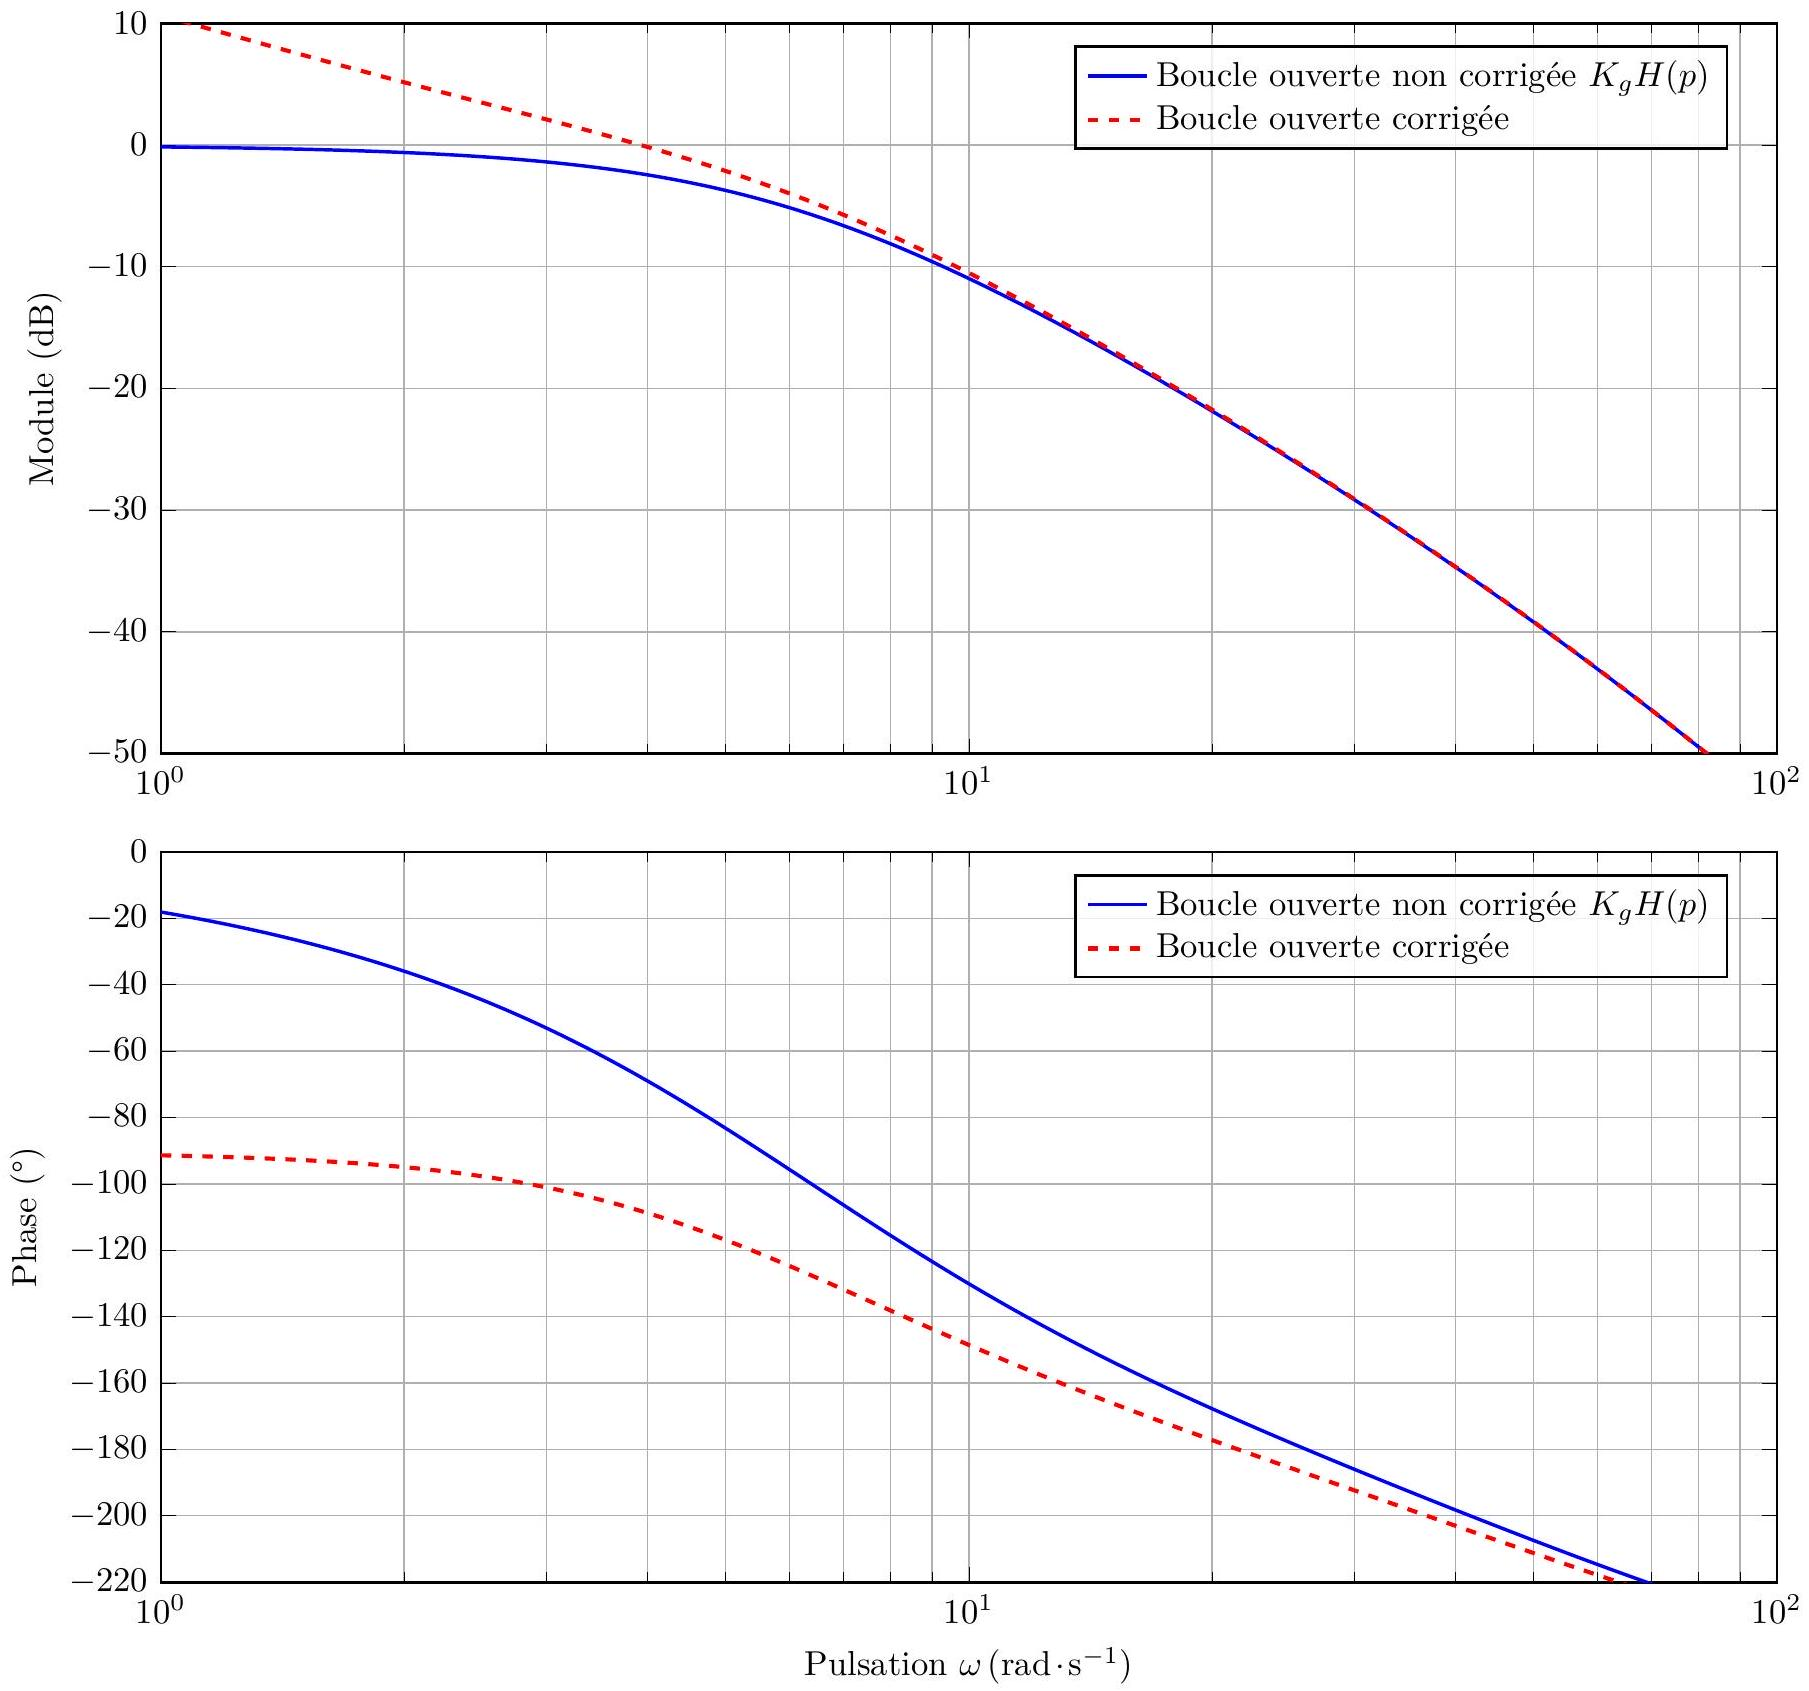
\includegraphics[alt={},max width=\textwidth]{5f5eb520-01ce-45b9-9641-42f0a6c20c83-12_1691_1809_127_149}
\captionsetup{labelformat=empty}
\caption{Figure 18 - Diagramme de Bode en boucle ouverte non corrigée $\left(K_{g} H(p)\right)$ et corrigée}
\end{center}
\end{figure}

Pour $T_{i}=0,3 \mathrm{~s}$ et la valeur du gain $K_{i}$ déterminée précédemment, les réponses obtenues en considérant respectivement des variations sur la vitesse du volant et de la masse de l'ensemble sont données sur les figures 19 à 21 de l'annexe 2

\begin{itemize}
  \item[-] la figure 19 montre l'évolution de l'angle $\beta(t)$ en réponse à une condition initiale d'amplitude $\beta(0)=0,1 \mathrm{rad}$ (cas d'une perturbation modifiant les conditions d'équilibre par exemple) pour une consigne nulle ;
  \item[-] la figure 20 montre l'évolution de l'angle $\beta(t)$ en réponse à une consigne d'amplitude 0,1 rad pour les valeurs nominale, minimale et maximale de la vitesse $\omega_{v}$ du volant du gyroscope;
  \item[-] la figure 21 montre l'évolution de l'angle $\beta(t)$ en réponse à une consigne d'amplitude 0,1 rad pour les valeurs nominale, minimale et maximale de la masse totale du scooter \{scooter + pilote + charge\}.
\end{itemize}

Q27. Commenter ces résultats au regard des performances attendues, exprimées par le diagramme d'exigences de la figure 3, en prenant en compte les différents critères d'analyse possibles (temps de réponse, amortissement, etc.).

Dans une étude prospective, et afin d'étendre les capacités de transport, il est envisagé d'utiliser ce système pour des masses totales jusqu'à 420 kg, soit une masse de l'ensemble $260 \mathrm{~kg} \leq M \leq 420 \mathrm{~kg}$. Il est alors nécessaire de vérifier la sensibilité de la loi de commande, calculée pour une masse nominale $M=280 \mathrm{~kg}$, à la variation de masse sur cette plage de fonctionnement.

Pour cette analyse le calcul des pôles en boucle fermée pour $260 \mathrm{~kg} \leq M \leq 420 \mathrm{~kg}$ est effectué avec des incréments de 10 kg. Les figures 22 et 23 de l'annexe 3 montrent les évolutions des pôles dominants dans le plan complexe en fonction de la masse

\begin{itemize}
  \item[-] la figure 22 correspond au cas de la commande sans action intégrale (schéma bloc de la figure 10);
  \item[-] la figure 23 correspond au cas de la commande avec action intégrale (schéma bloc de la figure 16).
\end{itemize}

Les droites iso-amortissement (lieux de points du plan complexe avec le même amortissement) sont tracées pour des coefficients d'amortissement $\xi \in\{0,3 ; 0,5 ; 0,7 ; 0,8 ; 0,9\}$.

Q28. Analyser les évolutions des pôles, figures 22 et 23, pour les différentes valeurs de la masse totale et commenter

\begin{itemize}
  \item[-] l'évolution des pôles dans le cas de la commande sans action intégrale (figure 22) et en particulier leur emplacement pour la masse nominale $M=280 \mathrm{~kg}$;
  \item[-] l'impact de l'introduction de la commande avec action intégrale sur les propriétés du système bouclé (évolution des pôles, coefficients d'amortissement, etc.) en s'appuyant sur la comparaison des pôles dans les deux cas ;
  \item[-] les performances de la loi de commande au regard du cahier des charges exprimé par le diagramme des exigences de la figure 3.
\end{itemize}

\section{Partie E - Synthèse}
En s'appuyant sur les écarts des niveaux de performances observés vis-à-vis de ceux attendus par le cahier des charges, il s'agit dans cette partie d'effectuer l'analyse globale de la pertinence du système de stabilisation active. Une évolution de la solution étudiée pourra être proposée de façon à respecter le cahier des charges pour des cas d'utilisation étendue permettant d'envisager une variation de la masse totale \{scooter + charge + pilote\} plus importante.

Q29. Analyser l'ensemble des réponses obtenues et conclure (en argumentant la réponse) sur la pertinence de l'architecture de commande retenue au regard des exigences du cahier des charges. En particulier, pour cette analyse faire apparaître distinctement les cas

\begin{itemize}
  \item[-] de la masse totale restreinte à celle définie par les exigences de la figure 3 ;
  \item[-] de la plage étendue $260 \mathrm{~kg} \leq M \leq 420 \mathrm{~kg}$ envisagée pour l'augmentation prospective des capacités de charge du scooter.
\end{itemize}

Q30. Proposer une évolution de la solution retenue en vue de satisfaire l'ensemble des exigences du cahier des charges sur l'étendue de la plage de masse.

\section{Opérations et fonctions disponibles en Python}
\section{Fonctions Python diverses}
\begin{itemize}
  \item[-] range(n:int) renvoie la séquence des n premiers entiers $(0 \rightarrow n-1)$ list(range(5)) → [0, 1, 2, 3, 4].
  \item[-] enumerate(s) itère sur la séquence s en renvoyant, pour chaque élément de s, un couple formé de son indice et de l'élément considéré list $($ enumerate $([3,1,4,1,5])) \rightarrow[(0,3),(1,1),(2,4),(3,1),(4,5)]$.
  \item[-] np.linalg.eig(A) calcule les valeurs propres et vecteurs propres d'une matrice carrée $A$, soit $A V=\lambda V$.
  \item[-] scipy.integrate.odeint(func, y0, t) résout numériquement un système d'équations différentielles ordinaires $\frac{d y}{d t}=f(y, t)$, où func est la fonction dérivée, y0 le vecteur des conditions initiales, et t le vecteur des temps.
  \item[-] np.linalg.solve(A,B) résout un système d'équations linéaires de la forme $A X=B$, où $A$ est une matrice carrée et $B$ un vecteur ou une matrice.
  \item[-] np.roots (p) calcule les racines d'un polynôme.
\end{itemize}

\section{Opérations sur les listes}
\begin{itemize}
  \item[-] len(u) donne le nombre d'éléments de la liste u $\operatorname{len}([1,2,3]) \rightarrow 3, \operatorname{len}([[1,2],[3,4]]) \rightarrow 2$.
  \item[-] u.count(e) renvoie le nombre d'éléments de la liste u égaux à e [1, 2, 3, 1, 5].count(1) → 2.
  \item[-] u + v construit une liste constituée de la concaténation des listes u et v $[1,2]+[3,4,5] \rightarrow[1,2,3,4,5]$.
  \item[-] n * u construit une liste constituée de la liste u concaténée n fois avec elle-même 3 * [1, 2] → [1, 2, 1, 2, 1, 2].
  \item[-] u[i] = e remplace l'élément d'indice i de la liste u par e.
  \item[-] $\mathrm{u}[\mathrm{i}: \mathrm{j}]=\mathrm{v}$ remplace les éléments de la liste u dont les indices sont compris dans l'intervalle [[i, j [[ par ceux de la séquence v (peut modifier la longueur de la liste u).
  \item[-] u.append(e) ajoute l'élément e à la fin de la liste u (identique à u[len(u):] = [e]).
  \item[-] u.extend(v) ajoute les éléments de la séquence v à la fin de la liste u (identique à u[len(u) :] = v).
  \item[-] u.insert(i, e) insère l'élément e à la position d'indice i dans la liste u (en décalant les éléments suivants); si $\mathrm{i}>=\operatorname{len}(\mathrm{u})$, e est ajouté en fin de liste (identique à u[i:i] = [e]).
  \item[-] del u[i] supprime de la liste u son élément d'indice i (identique à u[i:i+1] = []).
  \item[-] u.reverse() modifie la liste u en inversant l'ordre de ses éléments.
  \item[-] e in u teste si l'élément e apparait dans la liste u.
\end{itemize}

\section{Opérations sur les tableaux (np.ndarray)}
\begin{itemize}
  \item[-] np.array(s) crée un nouveau tableau contenant les éléments de la séquence s. La forme de ce tableau est déduite du contenu de s. np.array $([[1,2,3],[4,5,6]]) \rightarrow\left(\begin{array}{lll}1 & 2 & 3 \\ 4 & 5 & 6\end{array}\right)$.
  \item[-] np.zeros ((i,j),dtype=np.uint8) donne un tableau d'entiers à i lignes et j colonnes remplis de 0. Pour permettre au tableau de prendre des nombres complexes, changer dtype=np.uint8 par dtype=complex.
  \item[-] a.shape tuple donnant la taille du tableau a pour chacune de ses dimensions.
  \item[-] a @ b calcule le produit matriciel des deux tableaux a et b. Les dimensions de a et b doivent être compatibles.
  \item[-] a[i,j] = e remplace l'élément en ligne i et en colonne j du tableau a par e.
\end{itemize}

\section{Annexe n°2}
\begin{figure}[h]
\begin{center}
  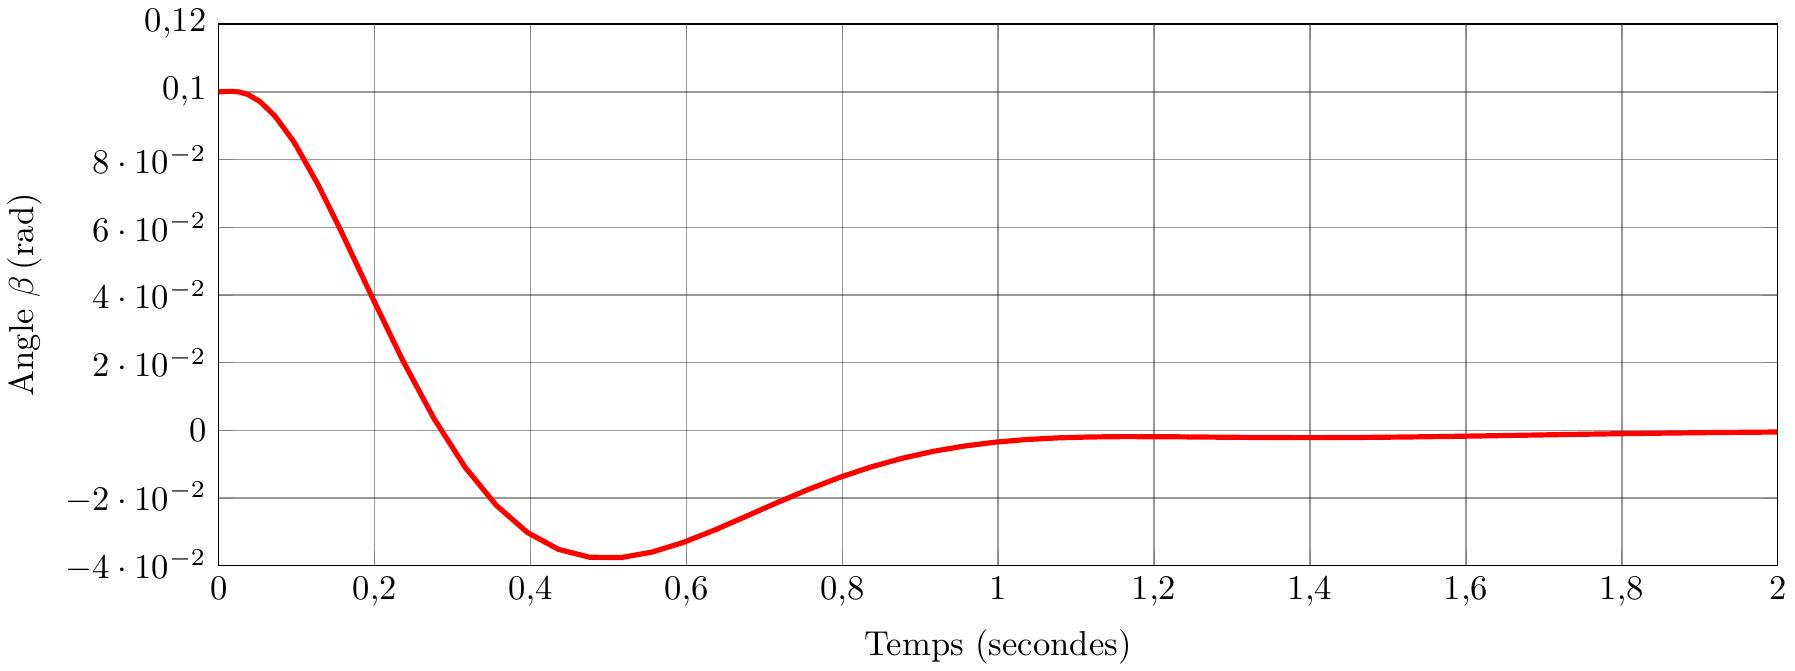
\includegraphics[alt={},max width=\textwidth]{5f5eb520-01ce-45b9-9641-42f0a6c20c83-15_671_1795_224_152}
\captionsetup{labelformat=empty}
\caption{Figure 19 - Réponse à une condition initiale d'amplitude 0,1 rad avec une consigne nulle}
\end{center}
\end{figure}

\begin{figure}[h]
\begin{center}
  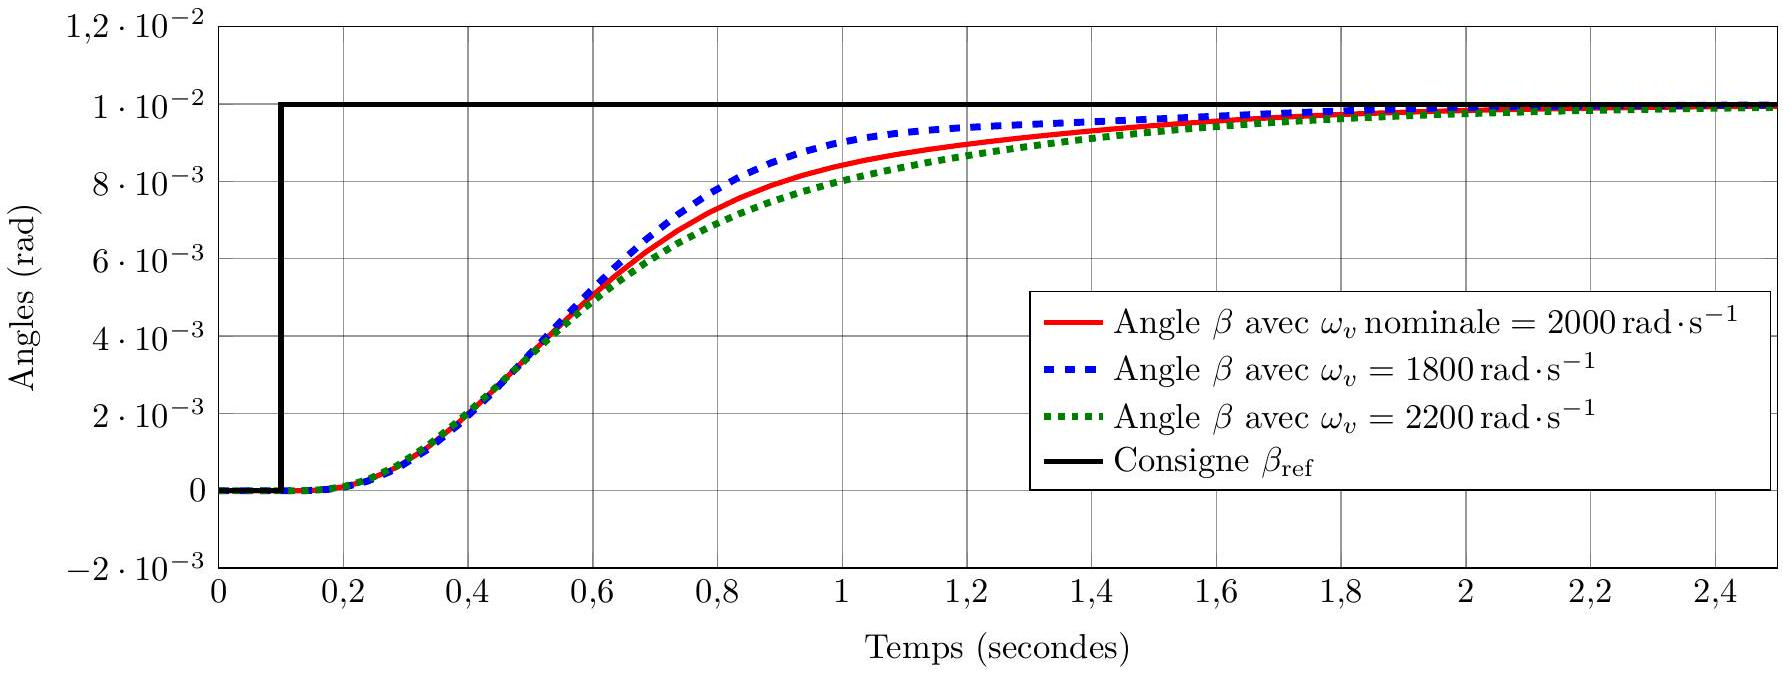
\includegraphics[alt={},max width=\textwidth]{5f5eb520-01ce-45b9-9641-42f0a6c20c83-15_674_1783_1058_152}
\captionsetup{labelformat=empty}
\caption{Figure 20 - Effet de la variation de la vitesse du volant du gyroscope $\omega_{v} \in\{1800 ; 2000 ; 2200\} \mathrm{rad} \cdot \mathrm{s}^{-1}$}
\end{center}
\end{figure}

\begin{figure}[h]
\begin{center}
  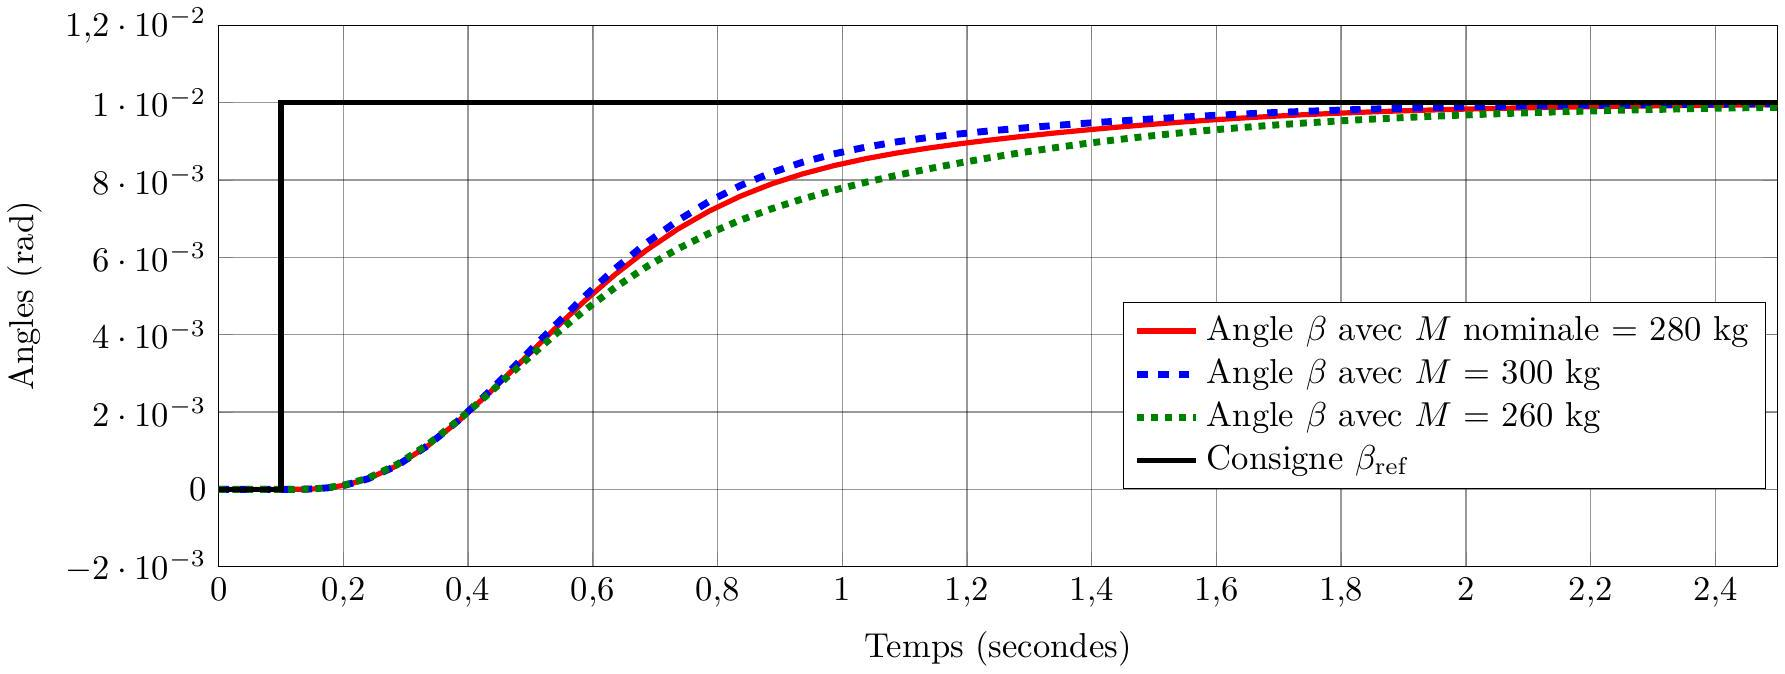
\includegraphics[alt={},max width=\textwidth]{5f5eb520-01ce-45b9-9641-42f0a6c20c83-15_674_1785_1896_152}
\captionsetup{labelformat=empty}
\caption{Figure 21 - Effet de la variation de la masse de l'ensemble $M \in\{260 ; 280 ; 300\} \mathrm{kg}$}
\end{center}
\end{figure}

\section{Annexe n°3}
\begin{figure}[h]
\begin{center}
  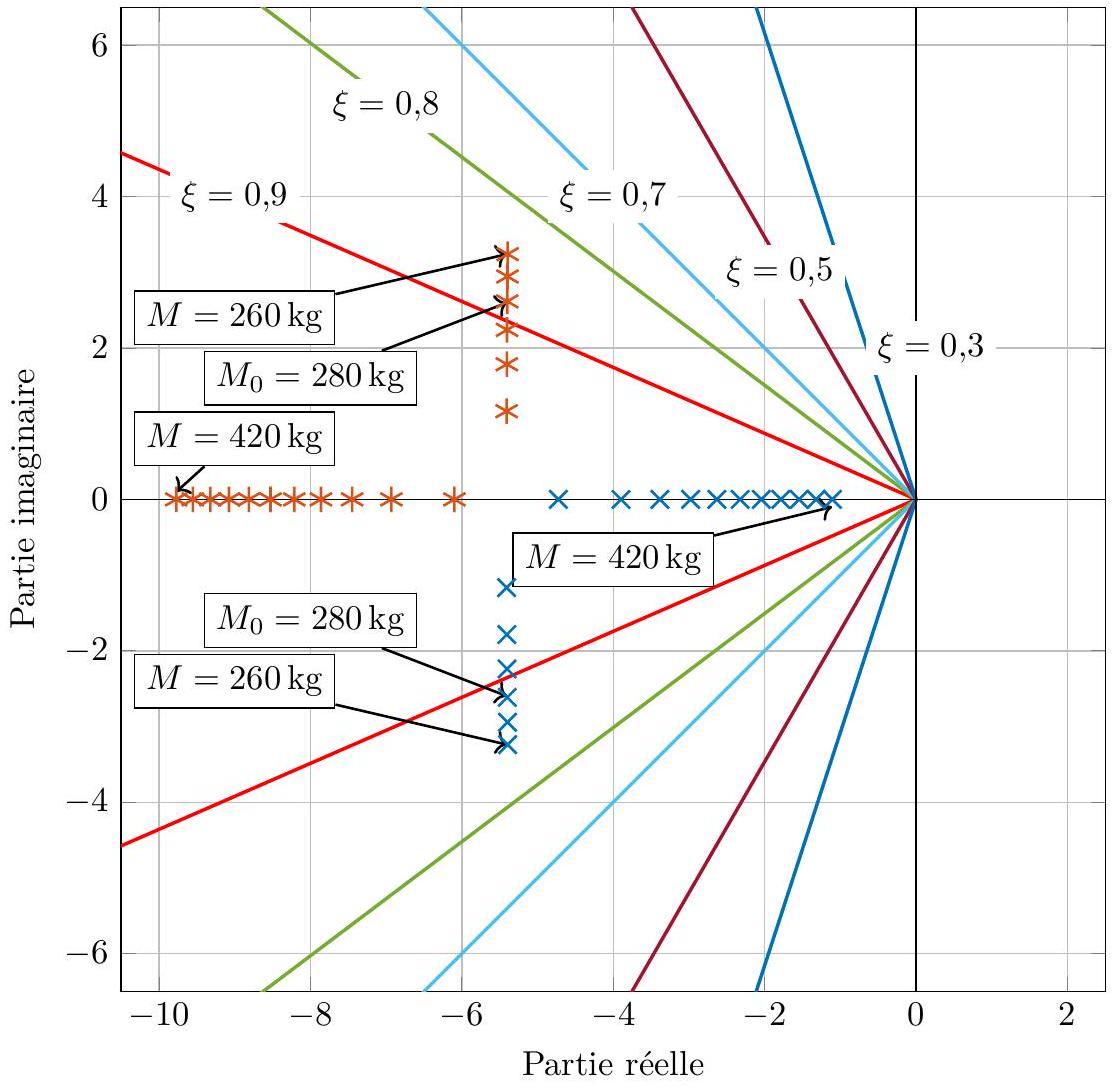
\includegraphics[alt={},max width=\textwidth]{5f5eb520-01ce-45b9-9641-42f0a6c20c83-16_1085_1114_214_481}
\captionsetup{labelformat=empty}
\caption{Figure 22 - Commande sans action intégrale (schéma bloc figure 10) : lieu des pôles (repérés par les symboles * et ×) du système en boucle fermée selon la valeur de masse de l'ensemble $260 \mathrm{~kg} \leq M \leq 420 \mathrm{~kg}$}
\end{center}
\end{figure}

\begin{figure}[h]
\begin{center}
  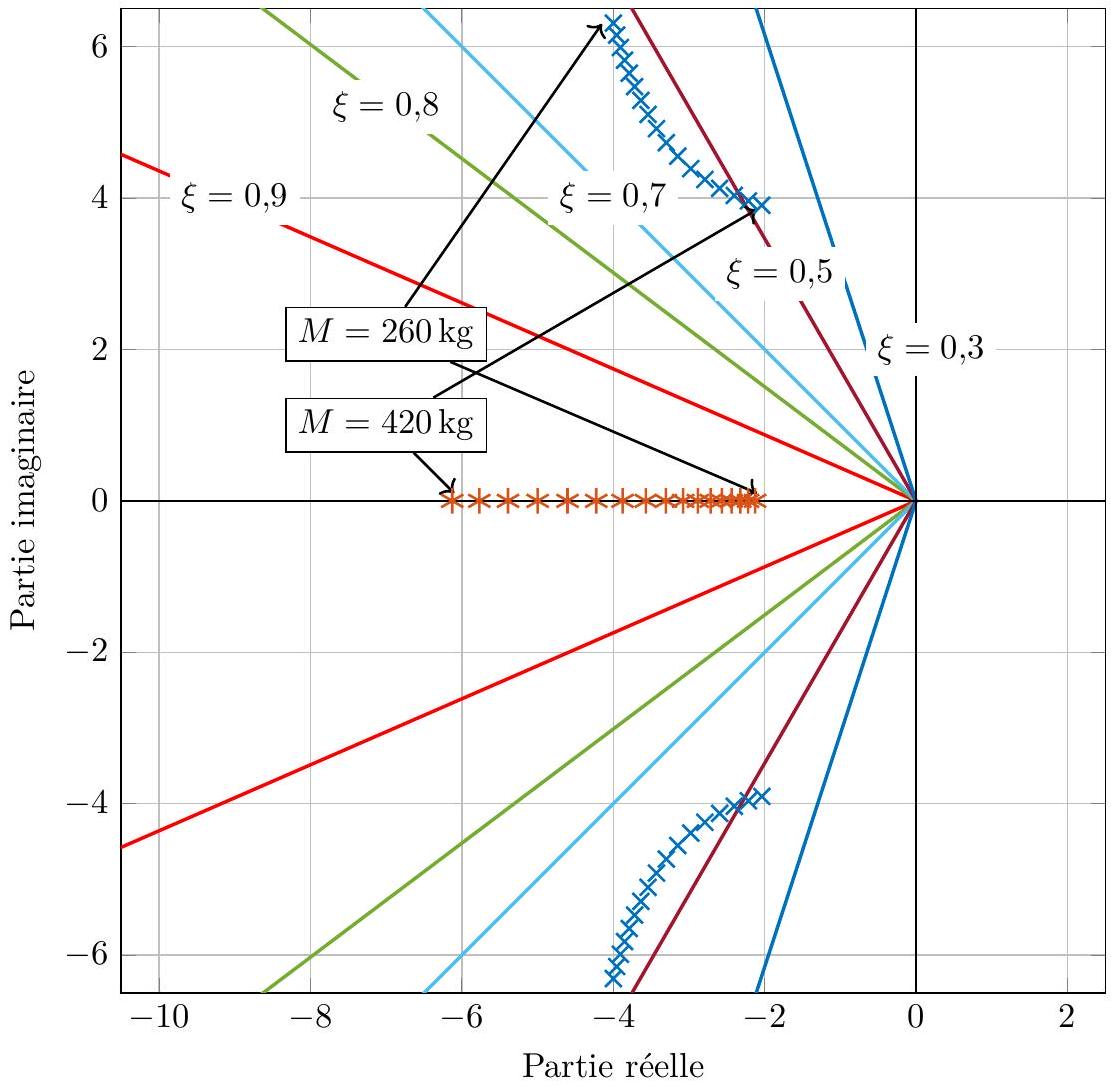
\includegraphics[alt={},max width=\textwidth]{5f5eb520-01ce-45b9-9641-42f0a6c20c83-16_1085_1111_1487_481}
\captionsetup{labelformat=empty}
\caption{Figure 23 - Commande avec action intégrale (schéma bloc figure 16) : lieu des pôles (repérés par les symboles * et ×) du système en boucle fermée selon la valeur de la masse de l'ensemble $260 \mathrm{~kg} \leq M \leq 420 \mathrm{~kg}$}
\end{center}
\end{figure}

\begin{enumerate}
  \item 
\end{enumerate}


\end{document}